\documentclass[a4paper,11pt]{kth-mag}
\usepackage[T1]{fontenc}
\usepackage{textcomp}
\usepackage{lmodern}
\usepackage[latin1]{inputenc}
\usepackage[swedish,english]{babel}
\usepackage{modifications}
\usepackage[acronym, toc]{glossaries}
\usepackage[colorlinks]{hyperref}
\usepackage{graphicx}
\usepackage{nameref}
%\usepackage{float}
\usepackage{wrapfig}
%\restylefloat{figure}
\usepackage{xcolor}
\usepackage[margin=10pt,font=small,labelfont=bf,
labelsep=endash]{caption}
%\usepackageappendix}
\usepackage{pdfpages}



\renewcommand\cftappendixname{\appendixname~} % Nicer look for appendixes in content list

\newcommand*{\fullref}[1]{\hyperref[{#1}]{\autoref*{#1} \nameref*{#1}}} % full reference including section/chapter tag
\newcommand*{\appfullref}[1]{\hyperref[{#1}]{Appendix \ref*{#1} \nameref*{#1}}} % full reference for appendices
\renewcommand*{\glsdisplayfirst}[4]{#1#4} % Glossary first entry

\newcommand*{\captionsource}[2]{%
  \caption[{#1}]{%
    #1%
    \\\hspace{\linewidth}%
    \textbf{Source:} #2%
  }%
}

\def\mypart#1#2{% 
\par\newpage\clearpage % Page break 
\vspace*{5cm} % Vertical shift 
\refstepcounter{part}% Next part 
{\centering \textbf{\Huge Part \thepart}\par}% 
\vspace{1cm}% Vertical shift 
{\centering \textbf{\Huge #1}\par}% 
\vspace{2cm}% Vertical shift % Some text 
#2 
\vfill\pagebreak %
}
\makeglossaries

% Epigraph
%\epigraphfontsize{\small\itshape}
\renewcommand{\epigraphrule}{0pt}
\renewcommand{\epigraphflush}{flushright}
%\renewcommand{\textflush}{center}
\setlength{\epigraphwidth}{.7\textwidth}

% Glossary
\newglossaryentry{rpi}{
name={Runaway Process Inflation}, 
text={runaway process inflation}, 
description={Runaway inflation is a very rapid inflation (decrease of money value). Runaway process inflation is a term sometimes used within agile development to describe rapidly growing development processes}}

\newglossaryentry{td}{
name={Technical Dept},
text={technical dept}, 
description={Technical dept (also called design dept or code dept), is a metaphor primarily used in software development referring to the consequences of poor system design. The dept builds up as you for example introduce bugs and so called spaghetti code that has to be fixed in the future, as in repaying your dept}}

\newglossaryentry{ev}{
name={Early Victory}, 
text={early victory},
description={A strategy commonly referenced to in agile development that refers to the sociological benefits of showing early and frequent results, such as increasing morale and trust}}

\newglossaryentry{osmosis}{
name={Osmosis},
text={osmosis}, 
description={The movement of a liquid, sometimes gas, through a plasma membrane (which is a sort of filter) which over time results in a balancing from high concentration areas to low for the molecules that are able to pass through the plasma membrane}}

\newglossaryentry{es}{
name={Executive Sponsor},
text={executive sponsor}, 
description={Also referred to as the project sponsor. Executive sponsor is a role in project management that is responsible to the business/company for the success of a project}}

\newglossaryentry{git}{
name={Git}, 
text={Git},
description={Git is a popular distributed revision control system mainly used for software development}}

\newglossaryentry{jitg}{
name={JIT}, 
description={Just-in-time is a production strategy that seeks to improve the \gls{roi} for a business by reducing in-process inventory and associated carrying costs. In simpler terms, reducing the stock up of inventory items in a process chain}}

\newglossaryentry{roig}{
name={ROI}, 
description={Return on investment means the benefits, or return, for the investor resulting from an investment of some resource. High ROI}}

\newglossaryentry{stake}{
name={Stakeholder},
text={stakeholder},
description={Has several meanings but this report refers to corporate stakeholders. A corporate stakeholder is a broad term meaning a person or party who has an interest in a certain business or project for a company. It can for example be investors, customers and suppliers}}

\newglossaryentry{us}{
name={User Story},
text={user story},
plural={user stories},
description={Within software development and product management, user stories are short descriptions, or stories, that tries to envision the users interaction for some requirement. The layout of user stories varies for different projects but It should capture the "who", "what", and "why" in a short but descriptive way. Usually the stories are highly abstract but before implementation on a story begins they are broken down into more fine graned sub-stories. The term is commonly used within agile development and originates from the methodology \gls{xp}}}


% Acronyms
\newglossaryentry{jit}{type=\acronymtype, name={JIT}, description={just-in-time}, first={just-in-time (JIT)\glsadd{jitg}}, see=[Glossary:]{jitg}}
\newglossaryentry{roi}{type=\acronymtype, name={ROI}, description={return-on-investment}, first={return-on-investment (ROI)\glsadd{roig}}, see=[Glossary:]{roig}}
\newacronym{tdd}{TTD}{test-driven development}
\newacronym{gui}{GUI}{graphical user interface}
\newacronym{wip}{WIP}{work-in-progress}
\newacronym{xp}{XP}{Extreme Programming}
\newacronym{lsd}{LSD}{lean software development}
\newacronym{lpd}{LPD}{lean product development}
\newacronym{dsdm}{DSDM}{dynamic systems development method}
\newacronym{uml}{UML}{unified modeling language}
\newacronym{css}{CSS}{cascading style sheets}



\title{Agile Development in a Solo Environment}


\begin{comment}


\subtitle{Duis autem vel eum iruire dolor in hendrerit in
          vulputate velit esse molestie consequat, vel illum
          dolore eu feugiat null}
\foreigntitle{Lorem ipsum dolor sit amet, sed diam nonummy nibh eui
              mod tincidunt ut laoreet dol}
              
              
\end{comment}              
              
              
\author{Mathias Lindblom}
\date{June 2015}
\blurb{Master's Thesis at KTH Royal Institute of Technology\\Computer Science and Communication (CSC)\\Supervisor: Sten Andersson\\Examiner: Olle B�lter}
 \trita{}
\begin{document}
\frontmatter
\pagestyle{empty}
\removepagenumbers
\maketitle
\selectlanguage{english}

\begin{comment}


\begin{abstract}
  This is a skeleton for KTH theses. More documentation
  regarding the KTH thesis class file can be found in
  the package documentation.

Lorem ipsum dolor sit amet, consectetuer adipiscing elit. Mauris
purus. Fusce tempor. Nulla facilisi. Sed at turpis. Phasellus eu
ipsum. Nam porttitor laoreet nulla. Phasellus massa massa, auctor
rutrum, vehicula ut, porttitor a, massa. Pellentesque fringilla. Duis
nibh risus, venenatis ac, tempor sed, vestibulum at, tellus. Class
aptent taciti sociosqu ad litora torquent per conubia nostra, per
inceptos hymenaeos.
\end{abstract}

\end{comment}


\clearpage

\begin{comment}

\begin{foreignabstract}{swedish}
  Denna fil ger ett avhandlingsskelett.
  Mer information om \LaTeX-mallen finns i
  dokumentationen till paketet.

Lorem ipsum dolor sit amet, consectetuer adipiscing elit. Mauris
purus. Fusce tempor. Nulla facilisi. Sed at turpis. Phasellus eu
ipsum. Nam porttitor laoreet nulla. Phasellus massa massa, auctor
rutrum, vehicula ut, porttitor a, massa. Pellentesque fringilla. Duis
nibh risus, venenatis ac, tempor sed, vestibulum at, tellus. Class
aptent taciti sociosqu ad litora torquent per conubia nostra, per
inceptos hymenaeos.
\end{foreignabstract}

\end{comment}

\clearpage
\tableofcontents*
\mainmatter
\pagestyle{newchap}

%\begin{comment}

\chapter{Introduction}
This chapter goes through the problem statement including goals, the target group and limitations. The last section will outline the structure of the rest of the report.

\section{Problem Statement}
Agile software development can be seen as a trend in today's computer industry. The variety of agile methodologies, as well as their definitions, changes frequently, which is quite appropriate given what agile development advocates. Most agile methodologies mainly targets established companies with advanced software systems. They talk about things like continuous improvement, rapid changes to new customer demands and the collaboration between self-organizing and cross-functional development using an iterative development process. However the information available regarding how-to practically establish an agile development process in small companies with small projects is limited. The available literature can give hints but has a strong focus on the full blown methodologies and leaves it up to the readers to decide what is practically possible for their limited sized development group or company.

The vast information available, complexity and focus on established companies can make it hard and confusing for developers wanting to adopt an agile mindset when starting their new company with only a few people or even by themselves. Trying to follow most agile methodologies completely, or other methodology types for that matter, would likely be overwhelming and lead to unnecessary early abandonment of that methodology. By finding a good approach to how small development teams and/or companies can adopt an agile development process, more companies/teams could benefit from the potential positive outcomes that comes from utilizing agile development.
%\section{Motivation \& Value} %syfte

\subsection{Goals}
The main goal of the thesis is as follows:

\begin{itemize}
\item Find an agile development methodology and potentially modify it to make it suitable for small development teams and/or companies consisting of 1-5 members.
\end{itemize}
\noindent
Secondary goals:

\begin{itemize}
\item Theoretical comparison of popular agile development methodologies suitable for small companies/development teams..
\item Overall clarification of agile terms and thinking/reasoning. For example differentiate Agile from Lean.
\item Produce a working prototype of the interactive tutoring framework described at \fullref{sec:project_description}.
\end{itemize}

\subsection{Target Audience}
The target audience are mainly small newly started IT companies with limited experience in software development methodologies. However, anyone having an interest in developing something using an agile approach, either alone or with a handful of people, might find this report useful. 

For those lacking prior knowledge regarding agile development, \fullref{sec:agile_development} together with \fullref{sec:agile_methodologies} should contain enough content to make the reader acquainted to the subject and understand the rest of the report. After all, given the target audience, it would be inappropriate not to offer the readers a comprehensive background.

\subsection{Limitations}
This report does not seek to investigate whether or not agile development as a whole is advantageous, compared to other methodology types, for small development teams. Instead it makes the assumption that agile development is advantageous and investigates what agile approach is most suitable for small development teams. 

The large scope of the agile development methodologies, the many social parameters and variety of projects means that the outcome of this report can't come to definite conclusions. It can't for example conclude that a certain methodology is the absolute best choice for small IT companies. This also explains the vague word \emph{suitable} in the goals section above. The report and investigation should instead be seen more as an thorough, experiential based and comprehensive guide. This is brought up again in \fullref{sec:discussion}.

\section{Thesis Outline}
Below are the chapters following the introduction of this report, in order, containing information about the flow of the report.

The report will begin by giving background about agile development in \fullref{sec:agile_development}. Following is \fullref{sec:agile_methodologies} which is a comprehensive walkthrough of a few agile methodologies and their practices. Some of these practices will be mentioned throughout the rest of the report.

In \fullref{sec:method_teori} after a short theoretical evaluation, of the agile methodologies from the prior chapter, one methodology is selected to be used in the project. Afterwards in \fullref{sec:the_project}, the project is described and how the selected methodology was used within the project. It will also contain information about the results of the project and the subjective experience for the members of the project.

Lastly the outcomes of the project is discussed and analyzed, in \fullref{sec:discussion}.


%\end{comment}

%\mypart{Background} {The following two chapters forms the base for the theoretical and practical part of this reports study. The first chapter explains agile development as a concept and its core ideas. The second chapter explains some of the most common agile methodologies, by mainly going through their practices.}

\chapter{Agile Development}
\label{sec:agile_development}
This chapter goes through agile development as a concept and highlights its core ideas and principles. It also explains the differences between agile development and the waterfall model as well as lean development.

Most developers have experienced the nightmare of working on a project and slowly witness the increasing number of bugs, errors and time when adding new functionality. In order to combat this disheartening scenario, developers tend to create constraints and routines around their activity, forming a development process based on prior mistakes. However big development projects can be complex and even though experienced based constraints helps, the problems remains and builds upon each other. One solution for this is to keep adding more constraints and routines. So the development process grows and grows and until the process itself becomes so cumbersome and advanced that it creates the problems it was designed to prevent, which was to avoid \gls{td} and increase efficiency \cite{key1}. 

This so called \gls{rpi} was common among big companies around the millennium shift and at the time it was a growing negative trend \cite{key1}. Software teams around the world experienced this, including a few industry experts calling themselves the Agile Alliance who sought to fight it \cite{key1}. The ideas that make up agile development were not new at the time but it was the Agile Alliance that formulated the underlying concepts that make up agile development. The report will come back to this at \fullref{sec:manifesto}.

\section{Component Abstraction}
\label{sec:abstraction_components}
It is common that agile development is directly compared to the waterfall model which is strange given how they situate on different abstraction levels. The Waterfall model is a software development methodology just like for example Scrum. Agile development on the other hand is not a followable methodology by itself. It is more of an ideology or perhaps a collection of methodologies. So how is it even possible to compare the two of them? The answer is that people are comparing the waterfall model to some popular agile methodology like Scrum or some common practices like sprints and standup meetings, indirectly claiming that these elements represent agile development as a whole. This leads to confusion and unfair comparisons. So before continuing reading about agile development it is a good idea to get a short overview of the components that make up agile development. Bare in mind that this is a simplified overview meant to give the reader a better sense of how agile development and the methodologies with its practices correlate to each other.

In Figure \ref{fig:agile_abstraction}, agile development have been dividid into four different abstraction levels. First we have the ideology that consist of the core ideas such as The Agile Manifesto and principles. This is basically what defines agile development, which will be explained at \fullref{sec:manifesto} and forward. Secondly we have the methodologies and strategies that fulfills some or all of the agile principles and philosophies. The third abstraction are the practices that make up the methodologies, similar to how the principles make up agile development. However, the practices are more practically applicable and at a much lower abstraction level. Lastly, at the forth abstraction level, we have the actual tools that are needed to make the practices a reality. These tools can be very simple such as a physical room for meeting practices or more advanced such as the xUnit framework for test-driven development.

The report will frequently talk about these different components so it is a good idea to keep a mental image of Figure \ref{fig:agile_abstraction}. Moreover, this report will refer to agile development as an ideology in order to not confuse it with its methodologies.

\begin{figure}[h]
  \centering
    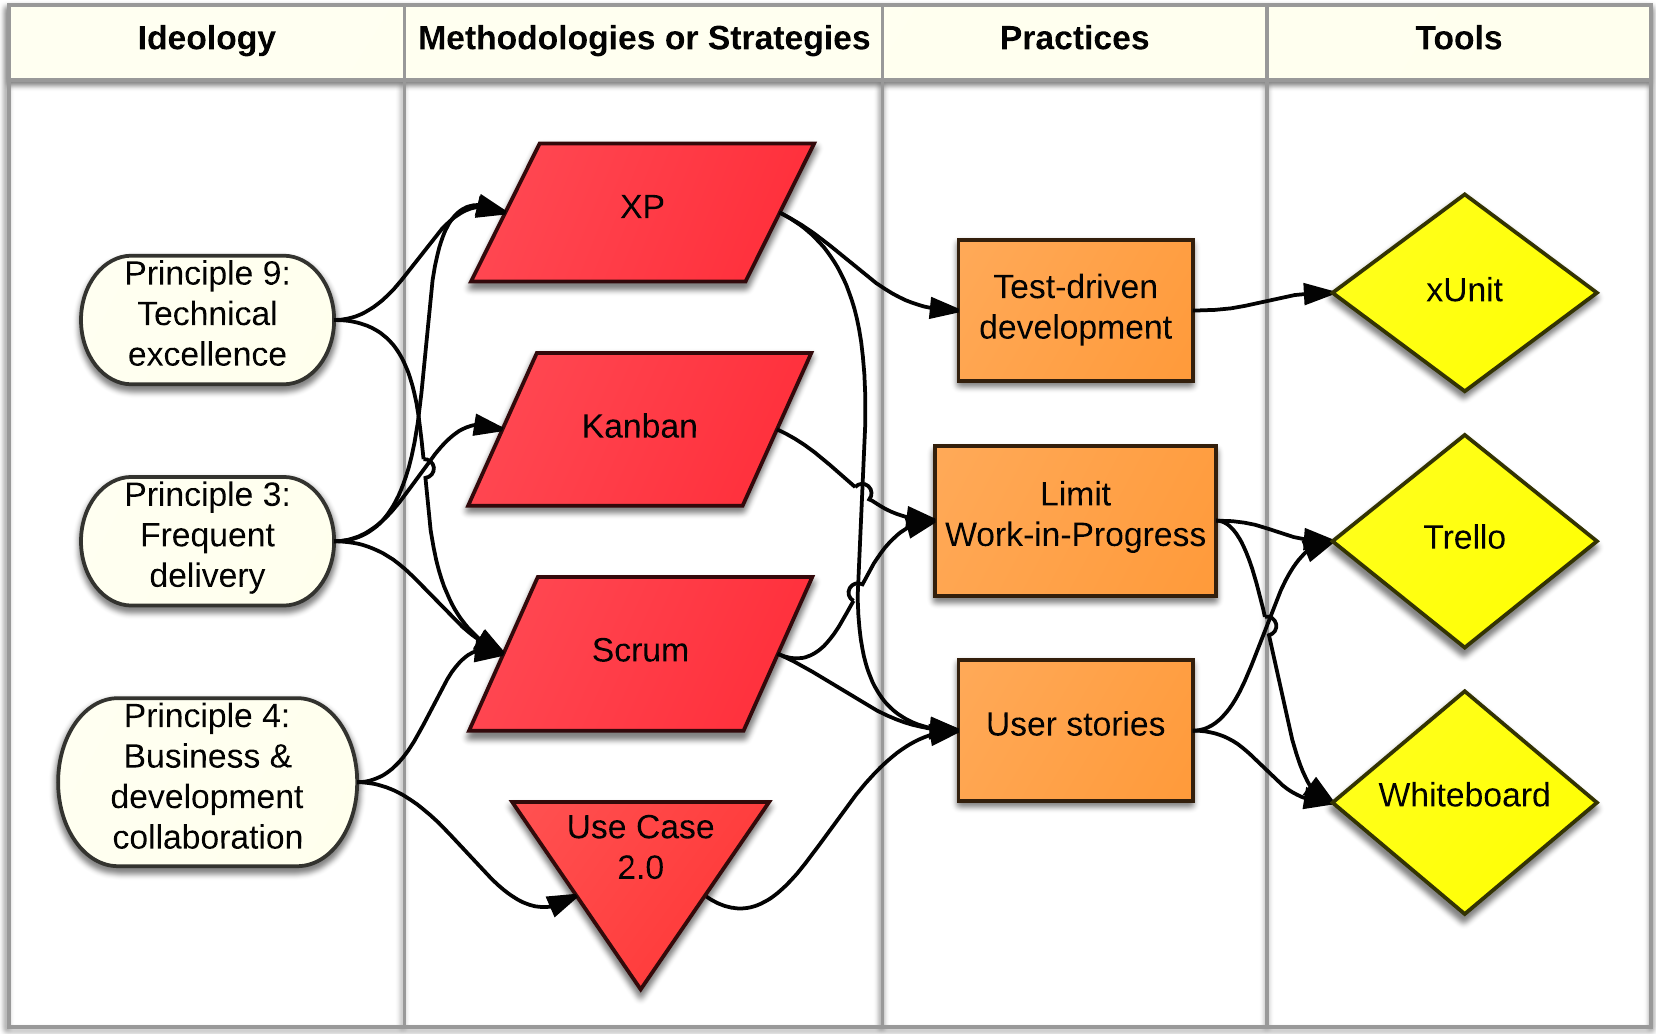
\includegraphics[width=1.0\textwidth]{img/agile_development_abstraction.png}
    \caption{Agile development divided into four different abstraction levels starting with the ideology that defines agile development and ending with physical tools. It also shows how the example elements within them correlate to each other.}
    \label{fig:agile_abstraction}
\end{figure}

\section{The Agile Manifesto}
\label{sec:manifesto}
The Agile Alliance is an organization formed by a group of computer industry experts in 2001. They decided to come together to form general development values in order to improve the software development process for companies around the world and to give an alternative to the popular heavyweight methodologies \cite{key1} \cite{key2}. The result was The Agile Manifesto that states the following:

\begin{itemize}
\item \textbf{Individuals and interactions} over processes and tools.
\item \textbf{Working software} over comprehensive documentation.
\item \textbf{Customer collaboration} over contract negotiation.
\item \textbf{Responding to change} over following a plan.
\end{itemize}

The group that wrote The Agile Manifesto consisted of the following people: \emph{Kent Beck, Mike Beedle, Arie van Bennekum, Alistair Cockburn, Ward Cunningham, Martin Fowler, James Grenning, Jim Highsmith, Andrew Hunt, Ron Jeffries, Jon Kern, Brian Marick, Robert C. Martin, Steve Mellor, Ken Schwaber, Jeff Sutherland, Dave Thomas} \cite{key1} \cite{key2}. Several of these people are the authors of the literature used in this report, this is especially true for \fullref{sec:agile_methodologies}.

The following four subsections will give a short explanation for each of the statements of The Agile Manifesto that stands as the highest abstraction or the core that is agile development. This will give the reader a good overview of the thinking and reasoning regarding agile development.

\subsection{Individuals and Interactions over Processes and Tools}

\epigraph{Process and technology are a second-order effect on the outcome of a project. The first-order effect is the people.}{\textsc{Alistair Cockburn} \cite{key1}}
\noindent
Within football most agree that a football team of average players that communicate well can beat a team of egoistic superstars. The same goes for software development (and probably many more things) where a team of average programmers working together outperforms a team of expert programmers that fail to communicate. At least according to the thinking and reasoning of agile development \cite{key1}.

Processes and tools are of course important as well but not as important. After all, agile development methodologies are processes that usually requires tools so it would be quite ironic otherwise. Team managers have a habit of setting up the development environment and then assigning a team, assuming that the team will work well since they have the tools they need \cite{key1}. However this is focus put at the wrong end of order. Tools and processes can rarely repair a team that doesn't play ball but a functioning team is usually more than capable of configuring their own environment.

\subsection{Working Software over Comprehensive Documentation}

\epigraph{The program is the specification and documentation.}{\textsc{Douglas Crockford} \cite{key3}}

\noindent
This might not be that much of a shocker, that functioning software is more important than documentation. The keyword here is \emph{comprehensive} since it is common that teams get hung up on the quest of having close to 100 percent coverage on documentation \cite{key1}. The problem with this is that it takes a lot of time and effort to always keep in sync with the code and as soon as you lose the sync, the documentation begins telling lies which is worse than having no documentation. Instead of having every technical part of a program described in a thick book it is usually preferred, both for the reader and the writer, to have a short rational and structured document that explains the software at a high abstraction. When a new member of a team needs more technical information they will get it when working closely and interacting with their team members and the actual software.

A common misconception is that code is for the computer and documentation is for the human to understand the code \cite{key4}. Instead of translating the code into human language, why can't we write code so that humans can understand it in the first place? We already do it by naming things like classes and methods with understandable names, but is usually ends there. We make it \emph{good enough}. If we instead focused more on the quality and logic of the code, the value of documentation would be greatly diminished. 

\subsection{Customer Collaboration over Contract Negotiation}
Many have tried to create strict contracts with fixed specifications, deadlines and prices for software development. Many have failed \cite{key3}. You simply can't treat software as a commodity expecting everything to be known before hand. Trying to do so can lead to all sorts of problems like poor quality or even complete failure. It is not only the complexity of programming that is the issue but also how fast our technical world changes over short time periods. 

This is one of the core problems that agile development tries to avoid. By having a tight collaboration with the customer, the specifications, deadlines and prices don't need to be as strict. Instead of having a contract specifying the exact requirements of the entire project it should instead address how the collaboration between customer and developers should be conducted \cite{key3}. This leads to a more dynamic development approach where technical problems can be addressed directly. Moreover, needed changes don't risk breaking the contract.

\subsection{Responding to Change over Following a Plan}	
The previous section regarding customer collaboration is an indirect example of this prioritization. Customers have a habit of not knowing what they really want or change their requirements after seeing some of the functionality coming to life \cite{key3}. Also like stated in the previous section, the IT world we live in rapidly changes and so can the requirements of a software project. It is nice and tempting to have the full project planned out in some advanced planning software with every functionality written. However as the development team and customer moves forward the plan is bound to change. Some functionality will no longer be deemed necessary and previously unthought of functionality might be added. Some parts of the strict plan might then have been a waste of time and more importantly, the strict plan might hinder these kind of changes that are needed or at least advantageous to the project. 

By having a more abstract and lose plan with details only for the near future, for example a couple of weeks, you get a planning more susceptible to change \cite{key3}. That detailed plan can be strict but since it is only for a short time period the risks of having unneeded functionality or hindering change is limited. The further away in time we look the weaker the plan should be since we want flexibility to changes and the likelihood of changing requirements grows as the timeline increases.

\section{The Agile Principles}
\label{sec:agile_principles}
Together with the values stated by The Agile Manifesto, 12 principles were created that act as the characteristics for agile practices \cite{key1}. You can interpret these principles as another formulation of The Agile Manifesto where you get a clearer explanation of what agile development means. These are the principles:

\begin{enumerate}
\item Our highest priority is to satisfy the customer through early and continuous delivery of valuable software.
\item Welcome changing requirements, even late in development. Agile processes harness change for the customer's competitive advantage.
\item Deliver working software frequently, from a couple of weeks to a couple of months, with a preference to the shorter timescale.
\item Business people and developers must work together daily throughout the project.
\item Build projects around motivated individuals. Give them the environment and support they need, and trust them to get the job done.
\item The most efficient and effective method of conveying information to and within a development team is face-to-face conversation.
\item Working software is the primary measure of progress.
\item Agile processes promote sustainable development. The sponsors, developers, and users should be able to maintain a constant pace indefinitely.
\item Continuous attention to technical excellence and good design enhances agility.
\item Simplicity--the art of maximizing the amount of work not done--is essential.
\item The best architectures, requirements, and designs emerge from self-organizing teams.
\item At regular intervals, the team reflects on how to become more effective, then tunes and adjusts its behavior accordingly.
\end{enumerate}


%\section{Misconceptions}
%Skeptics to agile development sometimes claim that agile development is just a trend, a so called fad. However the %arguments are similar to the time when people claimed the world wide web to be a youthful trend. It is a sort of straw man %argument based on that it is new and popular and will soon disappear, just like trends. 
%It is sort of a dictatorship vs democracy, dictatorship works but not well enough. And for a democracy to work the people %need to be onboard. 

\section{Agile vs Waterfall}
\label{sec:agile_waterfall}

 \begin{figure}[h!] % NOTE CHANGE TO WIDTH=1.0 IF POSSIBLE!
  \centering
    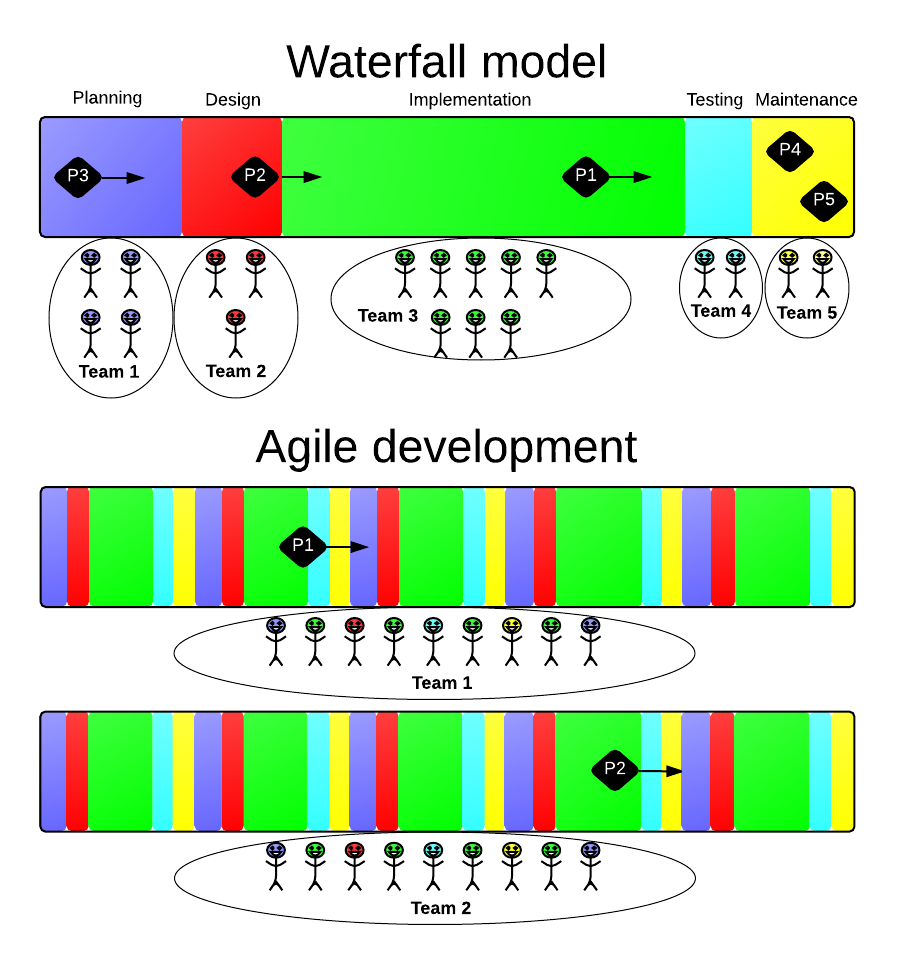
\includegraphics[width=0.9\textwidth]{img/agile_waterfall.png}
    \caption{Simplified highly abstract image showing the difference between the waterfall model and agile development. The image portrays how projects move forward in an arbitrary timeline through difference phases. P1 to P5 stands for Project 1 to Project 5. Each color represents a logical phase for a project such as planning or design. The stick figures represents team members and their color represents expertise within a certain phase. The image is further explained in \fullref{sec:agile_waterfall}.}
    \label{fig:agile_waterfall}
 \end{figure}
 \noindent
This section gives a short and illustrative view of the differences between agile development and the more established software development methodology called the waterfall model. As explained in \fullref{sec:abstraction_components}, one should be careful doing detailed comparisons between agile development and other methodologies since agile development is a bundle of methodologies. For this reason the comparison is held highly abstract.

As seen in Figure \ref{fig:agile_waterfall}, a project moves sequentially from one logical phase to the next in the waterfall model and rarely moves back to an prior phase. This means that once a project leaves a phase, it is assumed that that phase is completed for that project. Feel free to visualize a multi-step waterfall moving a log (project) from one water level (phase) to the next. The phases can hold different projects at any given time. Once a team in a certain phase is finished with a project, that project is moved to the next phase and the team is ready to receive a new project from the previous phase. All of this means for example that the implementation team does not care about design, or at least design is not their area of concern. In Figure \ref{fig:agile_waterfall}, when the design team is finished with project 2 (P2) it is moved to the implementation phase and the design team awaits the arrival of P3 from the planning team. 

Do note that the word \emph{team} is a simplification. In reality in the waterfall model, each phase can contain multiple development teams or so called functional units. The point is that each phase can be much more advanced than to simply contain a development team.

In agile development, the project does not normally move from one distinct phase to another. Instead, the project moves through layers of phases in a loop like fashion, as seen in Figure \ref{fig:agile_waterfall}. Another difference is that the same team holds a project until it is completely finished before starting to work on another project. In order to make that work it is vital that entire team incorporates all necessary skills within a project. A team that satisfies this is called a cross-functional team which are often mentioned within agile development. If another project starts, another cross-functional team is assigned that project. 



\section{Agile vs Lean}
\label{sec:agile_lean}
When you read about different software development methodologies they can sometimes be referred to as \emph{lean}, sometimes \emph{agile} and sometimes \emph{lean and agile}. Often without explanation of what specific parts makes the methodology lean and what makes it agile which can be very confusing. To understand the confusion it is best to give a short explanation of what lean development means:
\begin{description}
\item[Lean] \hfill \\
\Gls{lpd}, or lean manufacturing, dates back to the mid 20th century. The history of \gls{lpd} begins with Toyota that sought to improve car manufacturing efficiency, quality and flexibility. One way to achieve this, according to \gls{lpd}, is to have the entire chain from design to full assembly at one physical place \cite{key22}. This is comparable to how agile development promotes having short iterations where all parts of the software development chain is incorporated, as seen in Figure \ref{fig:agile_waterfall}. 

\Gls{lsd} is simply the adaptation of \gls{lpd} to the software industry that originates from the book  \emph{Lean Software Development: An Agile Toolkit} by Mary Poppendieck and Tom Poppendieck \cite{key23}. Like with agile development, \gls{lsd} has a few principles that gives a good overview of what the methodology framework or ideology is about:

\begin{enumerate}
\item Eliminate waste
\item Amplify learning
\item Decide as late as possible
\item Deliver as fast as possible
\item Empower the team
\item Build integrity in
\item See the whole
\end{enumerate}
\end{description}
 
Note that \gls{lsd} has just over half the amount of principles compared to agile development. Without going into detail for each specific principle we can see that several of the lean principles have similarities to the agile principles. L1 (lean principle number one) says to remove waste while A1 (agile principle number one) says to maximize value. L2 is hidden in several of the agile principles. L3 is about delaying decisions as late as possible to make the best informed decision which is a simplified version of A2. L4 and A3 both talks about fast delivery. L5 is basically what A5 states.

So by looking at the principles it is safe to say that the lean and agile ideologies have several similarities. They both talk about adaptive planning, empowering the people, fast delivery, continuous improvement etcetera. The differences lies in focus and scope that becomes more apparent when reading literature about them. \gls{lsd} focuses on minimizing waste and streamlining workflow while agile development focuses on adaptivity and communication. \gls{lsd} reaches a higher range than agile software development by going all the way to talk about costumer vision, staffing and maintenance while agile development has a more strict focus on the project development phase. 

What is important to note is that agile and lean do not go against each other. This means that methodologies trying to adopt these ideas do not have to be either agile or lean but can in fact be both, with perhaps a focus towards one of them. This chapter will end with a suitable long quote from one of the authors of The Agile Manifesto.

\epigraph{So as you can see, lean and agile are deeply intertwined in the software world. You can't really talk about them being alternatives, if you are doing agile you are doing lean and vice-versa. Agile was always meant as a very broad concept, a core set of values and principles that was shared by processes that look superficially different. You don't do agile or lean you do agile and lean. The only question is how explicitly you use ideas that draw directly from lean manufacturing.}{\textsc{Martin Fowler} \cite{key24}} 


\chapter{Agile Methodologies}
\label{sec:agile_methodologies}
Up to this point the ideology, that is agile development, has been described. In this chapter the more common methodologies that try to adapt these ideas and mentalities will be brought up. Moreover, the methodologies described here will contain more practically applicable agile practices. What is important to note is that every agile methodology is subject to change. Most authors and advocates of the agile methodologies encourages changes in the methodology itself to suit your development team and/or company. This means that the descriptions of the methodologies can look more or less different depending on the source, especially when they have been written years apart. Another reason is that some parts of a methodology can be vague resulting in different interpretations. However this does not necessarily mean that some descriptions of the practices are wrong. The vagueness can be seen as a way of encouraging changes and alternative implementations of the methodologies which the authors advocates.

The methodologies can be extensive in their documentation and this report does not seek to explain each methodology in their deepest details. That would simply require too much work and be overwhelming for the readers. For the interested reader, each methodology will have recommended further reading in its introduction.

One thing that every agile methodology has in common is a set of practices that explain the most important components. Some methodologies refer to them as properties but they all seek to explain the core of the methodology similar to how the agile principles, in \fullref{sec:agile_principles},  relate to agile development. It was therefor suitable to use them as the base for this reports overview of the methodologies in order to ensure that the description and comparisons are based on somewhat equal grounds.

A warning to the reader is that going through every practice of all four methodologies in order might be quite heavy reading. An alternative suggestion is to read the practice titles and go back to read the content when needed as the report starts investigating the practices at \fullref{sec:method_teori}. Note that whenever a practice is mentioned it is capitalized as a title.

\section{Scrum}
Scrum is one of the most known and used agile methodologies today. Scrum was originally codeveloped during the early 1990s by two of the soon-to-be authors of The Agile Manifesto, Jeff Sutherland and Ken Scwaber \cite{key21}. Several other mentionable people, such as Mike Beedle, have further contributed to the development of Scrum. Since the agile methodology Scrum was conceived just a few years before The Agile Manifesto and by several of the authors, it is perhaps not that shocking that people sometimes wrongfully put an equality mark between agile development and Scrum.

Scrum goes against the traditional predictive way of developing and instead has a more empirical approach. What this means is that Scrum assumes that problems and challenges can't be foreseen in software development. Therefor focus lies maximizing the Development Team's ability to deliver quickly and respond to changing requirements.

The information regarding the practices of Scrum is mainly taken from the book \emph{Agile Project Management with Scrum} by Ken Schwaber, one of the authors of The Agile Manifesto, together with updated information from the official Scrum web page: \url{www.scrumguides.org} \cite{key21} \cite{key15}. There are a total of 12 practices in Scrum divided the categories Roles, Events and Artifacts. Both the book and the web page are recommended for further reading regarding Scrum.

 \begin{figure}[h!] %NOTE, CHANGE TO WIDTH 1.0 IF POSSIBLE!
  
  \centering
    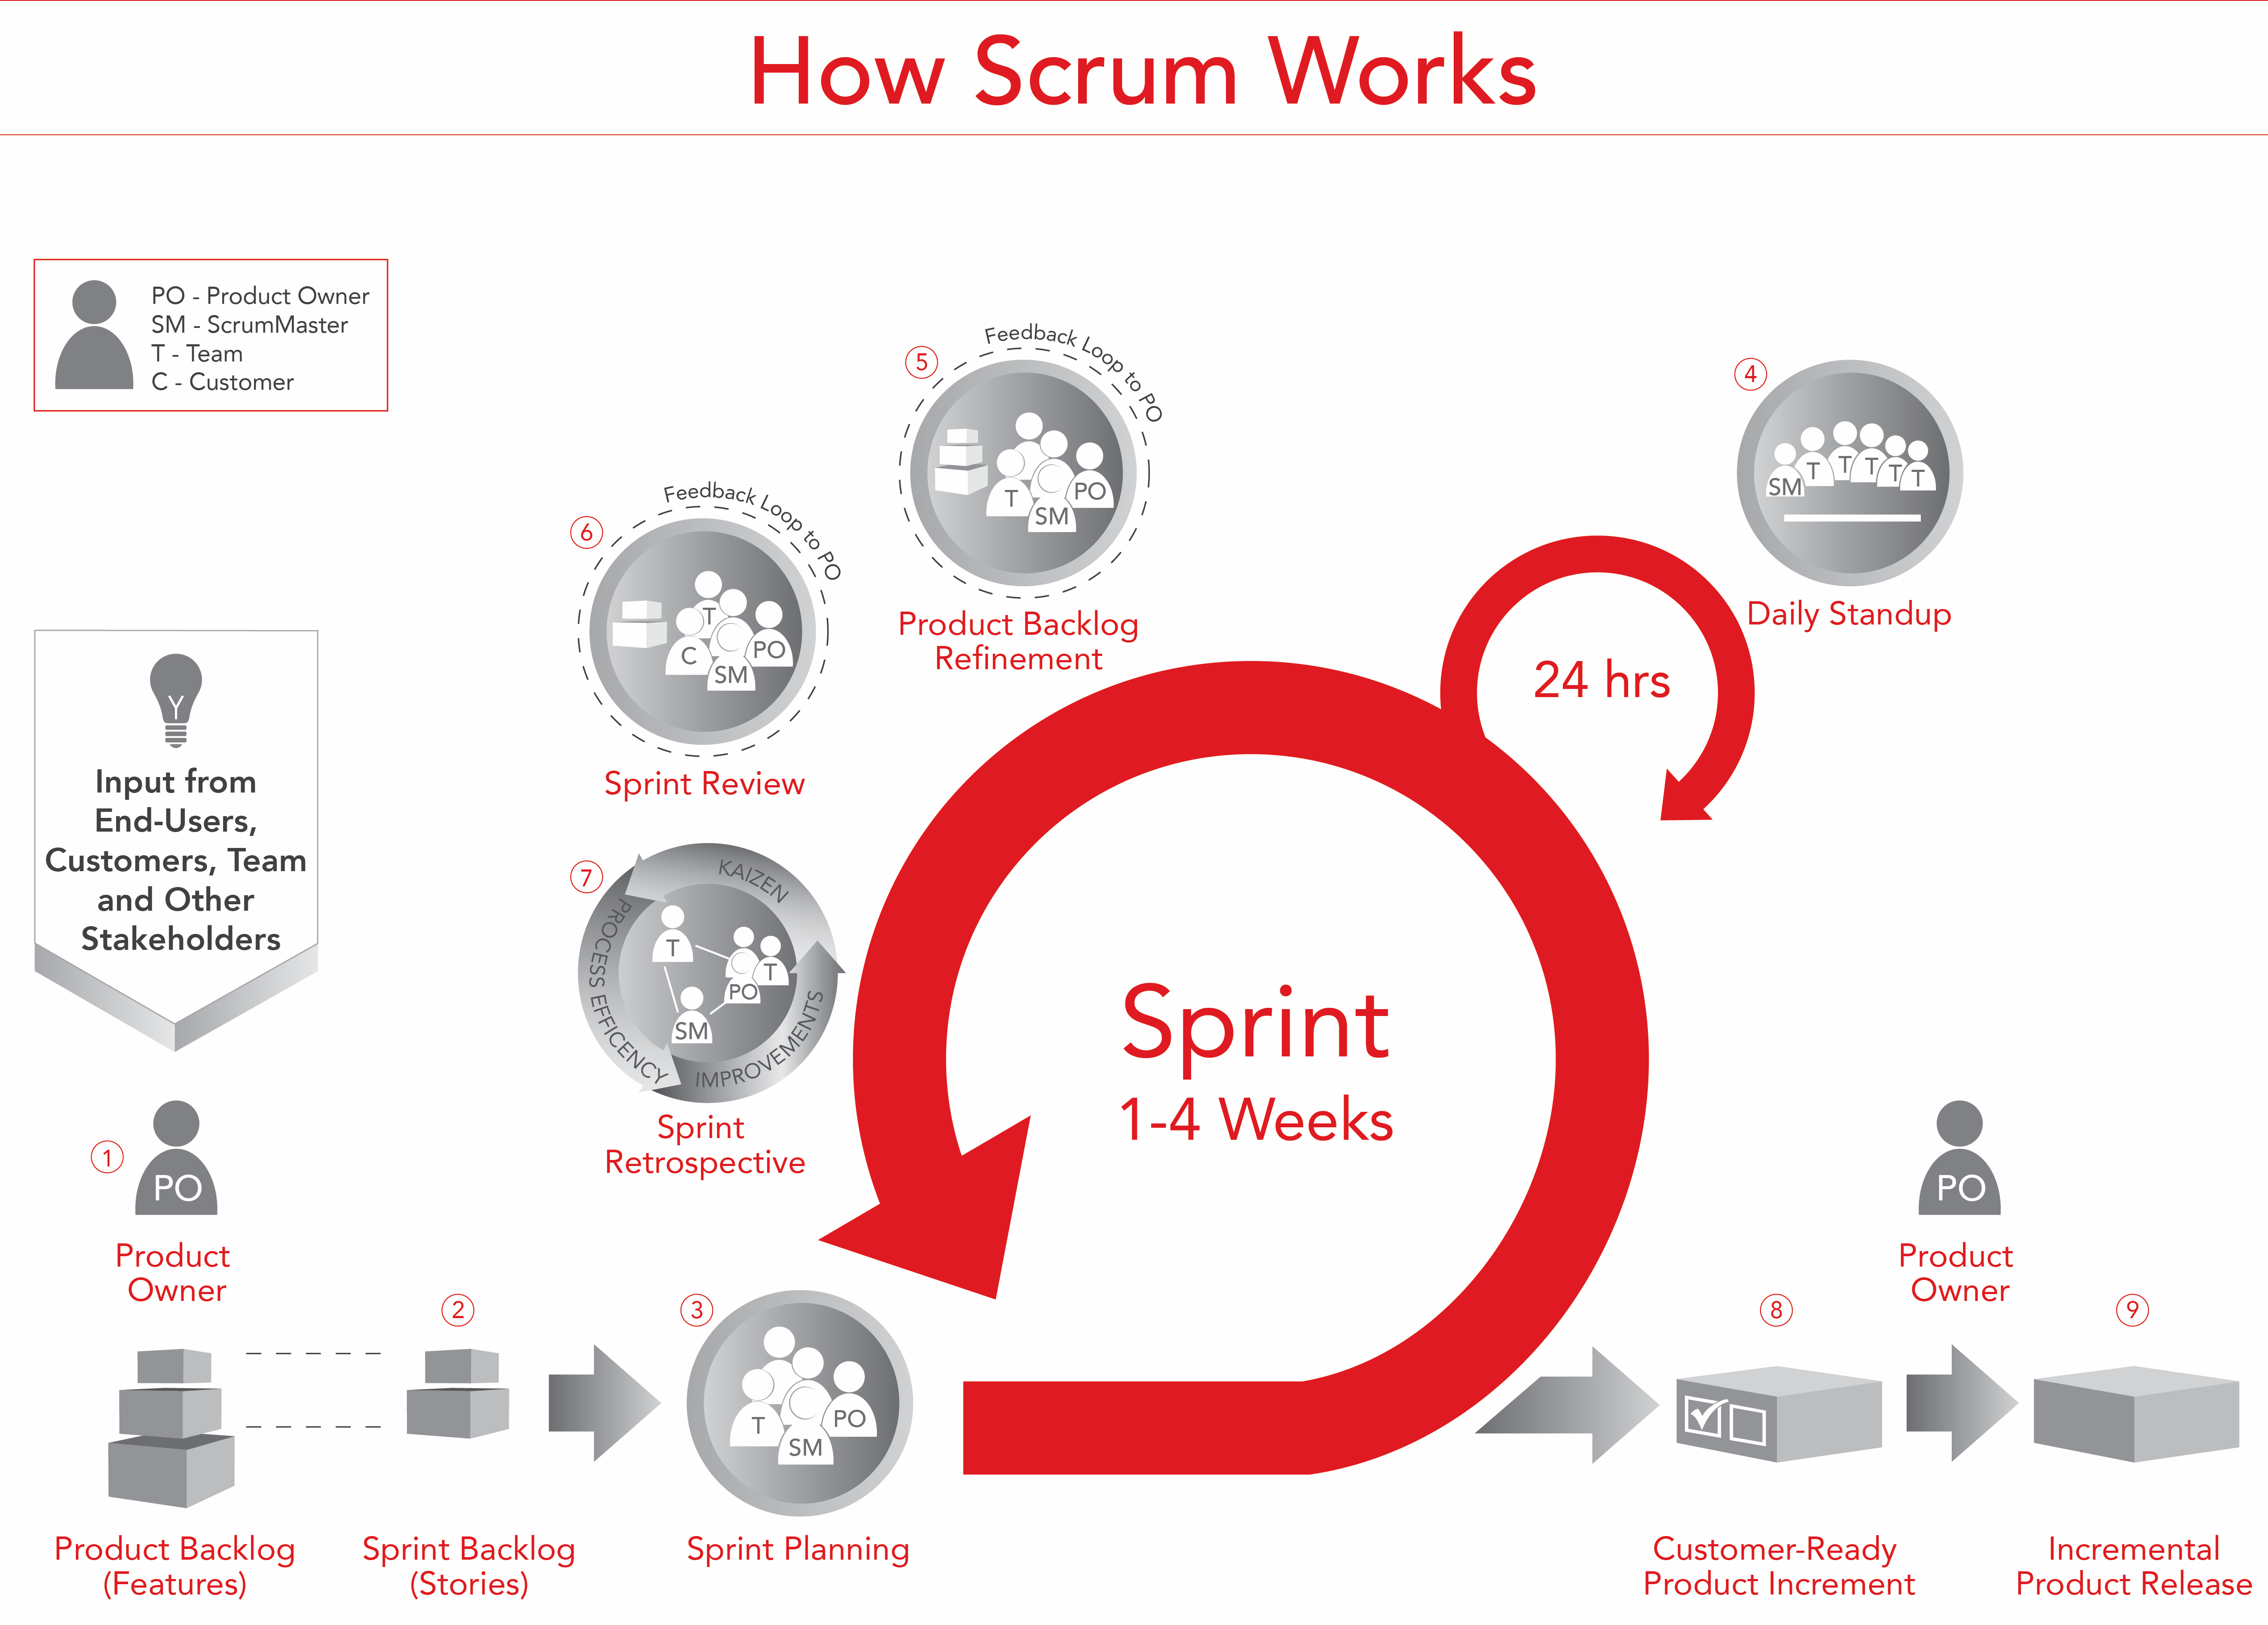
\includegraphics[width=0.88\textwidth]{img/how_scrum_works.png}
    \captionsource{Image showing an abstract view of how Scrum works, including different several practices including the three different roles.}{Scruminc, \url{http://www.scruminc.com}}
    \label{fig:scrum}
 \end{figure}

\subsection{Roles}
\label{sec:roles}
There are three distinct roles in Scrum. The Product Owner, Development Team and Scrum Master. The cooperation and relation between these roles is a key component in Scrum. The Scrum team consists of every member within these three roles.

\subsubsection{Product Owner}
The Product Owner is a single person. He/she is responsible of maximizing the work conducted by the Development Team which in turn means responsibility to maximize the product value. The practical priority is managing the�Product Backlog. The managing of the backlog means taking care of the following:

\begin{itemize}
\item Ensuring that the Product Backlog items have clear and distinct descriptions.
\item The ordering of backlog items to maximize value and reaching goals.
\item Optimization the value of the work by the Development Team.
\item Making the Product Backlog visible, transparent, clear to all project members and include information about upcoming tasks.
\item Having the Development Team on a satisfactory level of understanding of the items in the Product Backlog.
\end{itemize}

Depending on the size of the project and company. The Product Owner may choose to distribute some of the tasks to other people such as the Development Team. However, the Product Owner is always the accountable person for the above tasks \cite{key15}.

\subsubsection{Development Team}
In Scrum the Development Team are in charge of delivering working software, as one might expect. They are in a large sense self governed and chooses how they want to work, with some guidelines of course. 
The Development Team can be summarized with these characteristics:

\begin{itemize}
\item Self-organizing. The Development Team alone chooses how they want to turn the items in the Product Backlog into functionality.  
\item Cross-functional. The team should encompass all necessary skills to work with everything in the Product Backlog.
\item No titles within the group. Everyone is simply a developer.
\item No sub-teams. Just like there are no titles for the members, there can be no sub-teams such as a testing team. Not to be confused with multiple teams which is allowed and common in big projects.
\item All for one, one for all. Members might have specialized knowledge giving them natural areas of focus but the Development Team should always be accountable as a whole and never rely on individual expertise.
\end{itemize}

It is recommended that any Development Team consists of 3-9 members \cite{key15}. The reason being that too few developers limits the interaction and the team are more likely to have skill constraints. To many members lead to too much complexity that can make coordination between the members difficult.

\subsubsection{Scrum Master}
Deciding as a company to use a methodology and then explaining how the methodology works to all employees does not mean that the company will be developing according to that methodology. This is where the Scrum Master comes in. The Scrum Master is in charge of keeping the Scrum wheels turning. He/she makes sure that the Product Owner and Development Team are collaborating and generally doing what they are supposed to do. The following is a summarization of the responsibilities of the Scrum Master:

\begin{itemize}
\item Remove barriers regarding development so that the Product Owner is free to directly drive development forward.
\item Teach the Product Owner how to maximize \gls{roi} in order to meet his/her milestones using Scrum. 
\item Improve the quality of life for the Development Team by empowering them and encouraging creativity.
\item Assist the Development Team in increasing productivity in any way possible.
\item Ensure that each increment of functionality is potentially shippable by improving engineering practices and tools.
\item Give transparency to the Development Team's work progress for all parties and ensure it is up-to-date. 
\end{itemize}

The position of the Scrum Scrum Master is normally filled by the project manager. Ken Schwaber indicates in his book, \emph{Agile Project Management with Scrum}, that a Scrum Master should be a leader figure and never act as a regular boss \cite{key21}. 

\subsection{Events}
\label{sec:scrum_events}
In Scrum there are five so called events. However the first event called Sprint is the most important one and all the other events are basically a part of the Sprint.

\subsubsection{Sprint}
As seen in Figure \ref{fig:scrum} the Sprint is very central in Scrum. The Sprint is a short period of time, usually a couple of weeks up to a month \cite{key21}. As soon as one Sprint ends, another starts. The Sprint is about dividing the entire project into small iterations. The length of a Sprint should be small enough to avoid complexity but large enough to avoid too much project overhead. The following four practices are all parts of the Sprint and describes more in detail what the Sprint is about.

\subsubsection{Sprint Planning}
Each newly starting Sprint is initialized with a Sprint Planning. The entire Scrum team should be present during this planning. The Product Owner brings up the Product Backlog and its priorities. These are discussed by all parts and the Development Team goes through what will be achievable for the next Sprint. So to summarize the planning is about deciding what should be done and what can be done for the coming Sprint. The meeting usually has a time limit of 8 hours \cite{key21}.
\subsubsection{Daily Scrum}
Also referred to as daily standup as seen in Figure \ref{fig:scrum}. This is something that the Development Team does every day and should take around 15 minutes \cite{key21}. They do this to synchronize and coordinate their work efforts. There are three important questions to be answered during this meeting which are: What work have each member done since the last Daily Scrum? What is everyone planning on doing before the next Daily Scrum? What hinders exist that stand in the way of the team meeting the current Sprint goals? It is the Scrum Master's job to enforce that the Daily Scrum takes place and that it is only the members of the Development Team that participate \cite{key15} \cite{key21}.
\subsubsection{Sprint Review}
The Sprint Review is held close to the end of a Sprint. The entire Scrum team should be present and if possible the \glspl{stake} as well. This is supposed to be an informal meeting where the added functionality from the latest Sprint is shown. The Development Team shows what they have done and the Product Owner shows what has happened to the Backlog. The idea is to have a revised Product Backlog at the end that can be used for the next Sprint. The durations of this meeting is usually limited to four hours \cite{key21}.
\subsubsection{Sprint Retrospective}
The Sprint Retrospective should take place after the Sprint Review but before the upcoming Sprint Planning. Once again the entire Scrum team is present, but without the \glspl{stake}. This meeting should take about three hours \cite{key21}. The focus of this meeting is to improve the work process during a Sprint. The team reflects about things like tools, relationships, processes and anything else that can improve the workflow of the team and next Sprint.

\subsection{Artifacts}
The three artifacts are the most basic parts in Scrum that are worked on during the different events.

\subsubsection{Product Backlog}
The Product Backlog is the dynamic requirements list in Scrum. It is an item list comprising of anything that can add any form of value to the product. Typical items in a Product Backlog are new features, bugs, enhancements and functions. Each Product Backlog item also has certain attributes such as a description, priority order, complexity estimate and value estimate. 

What separates a Product Backlog from a simple requirements list is that it is a dynamic process and not a static list. The items in the Product Backlog that are to be considered for the "near future", as in having a high priority order, have more details than other items. This is to allow changes to the distant Product Backlog items as the actual product developes.  The Product Backlog is in focus for both the Sprint Planning and Sprint Review. The refinement of the Product Backlog items is sometimes counted as a practice by itself as seen in Figure \ref{fig:scrum}. However the items can be tuned and refined at any time. All members of the Scrum team have a saying when it comes to the Product Backlog but the Product Owner is the main responsible person.

\subsubsection{Sprint Backlog}
The Sprint Backlog is the selected items from the Product Backlog for the ongoing Sprint. It is the list of work to be done during the Sprint. All items in this backlog have clear details since the idea is to have them all completed at the end of the Sprint, which is a relatively short time period. The Sprint Backlog changes during a Sprint as the items become implemented and moved to "done". New items can also be added as unforeseen needed functionality is added. It is the Development Team that work with the Sprint Backlog and uses it as their progress report and todo list for the current Sprint. At each Daily Scrum the Sprint Backlog is updated and refined with informations such as remaining work hours. 

\subsubsection{Product Increment}
A Product Increment is the sum of all implemented Sprint Backlog items for a Sprint. It is a sort of "next step" for the product. The requirements for an item to be counted in the Product Increment is that it is fully usable for the product, regardless if the Product Owner chooses to release it or not.


\section{Extreme Programming (XP)}
\glsreset{xp}
Kent Beck is the founder of \gls{xp}. He is also one of the members of the Agile Alliance that you can read about at \fullref{sec:manifesto}. \gls{xp} was conceived shortly before the creation of the Agile Alliance. In 2000, just a year before the Agile Alliance surfaced, the first book about \gls{xp} called \emph{Extreme Programming Explained: Embrace Change} was published by Kent \cite{key14}. For this reason, when reading early literature about \gls{xp} their is no mentioning of the term \emph{agile}, which is  not strange since at the time the term did not exist. However more published articles and books have surfaced after the year of 2001 that have incorporated the agile ideology, such as the second edition of Kent's first book released in 2005 \cite{key14}.

Unlike Scrum, \gls{xp} almost solely talk about the developers and helping them be as efficient as possible. It does not talk much about the overall business outside the development team. Although if you read further about \gls{xp} you will find business related information but it is not at all in focus. \gls{xp} put emphasis on team work, feedback and code quality. The term extreme comes from the idea that it takes a few ordinary development practices and impose them to an extreme. Originally \gls{xp} was designed for small to medium sized teams but has over time grown to incorporate large teams as well. 

There are a total of 12 main practices in \gls{xp} that will be shortly described in the following sections. There are several corollary practices as well that talk more about the business and goes even further into coding details. To read about this and much more, the second edition of \emph{Extreme Programming Explained: Embrace Change} is recommended \cite{key14}.

\subsection{Fine-Scale Feedback}
The following practices describes how the members of the team develop their software with feedback in focus. It goes through the basics of how they work in pairs and always use \gls{tdd} to guide them. It also describes the relations between business people and developers.

\subsubsection{Pair Programming}
This is perhaps the most notable practice regarding \gls{xp}. Pair Programming means that for each developer, there is a another developer observing and assisting without coding. They work together similar as in rally racing where one person is the driver and one is the map reader. The main difference is that in Pair Programming the coders switch places regularly. The purpose is that the observing developer can have their mind set on a higher abstraction level and is not distracted by coding, making it easier to ensure high code quality \cite{key1}. Not only are bugs detected more easily but the overall resulting code is simply put better. This way of developing can be quite motivating for the developers since you are never alone and if you grow tired of typing you just switch places with your pair. If the developers also switch partners every other day, information and knowledge is spread rapidly and smoothly within the entire team. This is especially good when you have specialists with knowledge that could benefit the other developers. Studies conducted by Williams and Nosek has suggested that pairing does not reduce the development efficiency but does show a decrease in defect rate in the software \cite{key11}.

\subsubsection{Planning Game}
The Planning Game is played between the business people and the developers. It is about figuring out and deciding witch features to implement and basically form a prioritization of what needs to be done. The business people focuses on the importance of each feature \cite{key1}. The developers focuses on the cost of developing the features. 

A simple and natural way to play the game is: After each iteration, which for example might be a two week period, the developers updates the cost of future features. They also come up with a budget for how much they will be able to develop for the next iteration. Then it is the business peoples turn. They decide the features, within the budget, that they want the developers to work on for the next iteration. This game plays out after each iteration.

In reality it is much more complicated and a whole chapter is dedicated to the Planning Game in the book \emph{Agile Principles, Patterns, and Practices in C\#} by Martin C. Robert  and Martin Micah \cite{key1}. Things like velocity and \glspl{us} are described in detail which are all important components to the Planning Game. What is stressed is transparency since everybody might not be up to play ball just relying on some developers estimation. 

\subsubsection{Test-Driven Development}
The following steps describes \gls{tdd}:

\begin{enumerate}
\item Write an unit test for some functionality.
\item Make sure it fails before implementing it, since it would be strange otherwise.
\item Write the code that implements the functionality.
\item Run the unit test and if it fails, fix it until the test passes.
\item Repeat for every future functionality.
\end{enumerate}

This can seem overwhelming at first but it leads to having a close to 100 percent test coverage which can be very beneficial as the project grows. Another positive aspect is that writing test cases before coding leads to all code being testable by definition. Some may think: \emph{Isn't all code testable?} As soon as you build a system without the slightest thought about testability you will get the answer. Further more, using \gls{tdd} you tend to get code that is less coupled and better structured \cite{key1}. The reason for this is simply because your mind is set to create code that can be tested independently, indirectly leading to decoupled module like structure.

\subsubsection{Whole Team} 
Saying that \gls{xp} focuses on the entire team does not simply mean the entire development team. Everyone that is in any way connected to the \gls{xp} project should be collaborating closely with each other to solve problems. This goes as far as preferably having the customer in the same room or within 100 meters from the developers \cite{key1}. The more time the customer can spend with the team and the shorter distance the customer is from the team the better. If the customer is unable to be within close vicinity then it is advisable to have a stand in representant for the customer.


\subsection{Continuous Process}
These practices describes the cycles such as sprints and release plans for the project. Things like frequent integration are brought up and the importance of continuous refactoring. 

\subsubsection{Continuous Integration}
For those that frequently work with multiple people using \gls{git}, Continuous Integration will sound familiar. Each programmer should integrate their work several times a day. If you are lucky (or fast), you are first and simply check in your work. If you are not so lucky, you have to merge the changes. In other words, \gls{xp} teams use nonblocking source control \cite{key1}. This means that every developer can work on any part of the system, simultaneously with the other developers. It is important that each system test and acceptance test are run before anything is checked in. If something is broken, the developer fixes it before checking in the changes. 

\subsubsection{Refactoring}
Refactoring is not a backup practice when quality ensuring practices fail. Refactoring is a quality ensuring practice.

Sometimes it can be hard to convince non-programmers the benefits of refactoring. The main reason is that feature wise, nothing is added. At most some optimization might be noticeable. Refactoring is about changing the foundation of the software. It is to make adding new features a simpler task. Code duplication is a sign that refactoring is needed. When developers start to choose bad coding practices simply because they see no other way of implementing something, factoring is needed. When changing code affects unrelated code sections, refactoring is needed. However the idea is not to code poorly, fix it with refactoring and continue. Most developers knows that coming to a situation where refactoring is advisable is pretty much unavoidable, the important thing is not to add fuel to the flames. Pair Programming for instance seeks to diminish the need of refactoring and make sure quality is ensured \cite{key14}.

In \gls{xp} refactoring is not something you do only at the end of an iteration or cycle, not even something you only do at the end of the day. You do it as soon as you see that it is needed. This means that refactoring will come in really small packages that alone do not bring much value. Together however, all the refactoring keep the clone clean, simple and as expressive as possible.

\subsubsection{Small Releases}
Small Releases means release often and release small. Releasing software can be a pain but that is usually the case when you seldom release, thus having no routine for it. The releases in \gls{xp} can be split into two types. The iteration plan and the release plan:

\begin{description}
\item[The iteration plan] \hfill \\ 
This is a sort of minor release. In \gls{xp} the usual interval for minor releases of new software is every two weeks \cite{key1}. However as short as possible is preferred. The two week period is just a well working standard. At the end of each iteration cycle, decisions regarding \glspl{us} and features should be made according to the the Planning Game. It is not obligatory that something gets released at the end of this cycle since the short time period might mean that too few features with value have been implemented.  
\item[The release plan] \hfill \\ 
This is basically the bigger version of the iteration plan. This is a more abstract plan over a longer time period that usually spans around three months \cite{key1}. A clear difference is that the iteration plan should not change but the release plan is subject to change during its lifetime. A simple explanation for this is that it is expected to foresee
implementation issues two weeks ahead while this is not the case for three months. It is also expected that something gets released at the end of a release plan cycle.
\end{description}


\subsection{Shared Understanding}
The following practices  are about giving the developers a team feeling and shared understanding of the entire project. The practices talk about code design, abstraction and that sharing knowledge is caring.

\subsubsection{Coding Standards}
Pair Programming describes how knowledge can be spread swiftly by routinely changing programming partner. For this to work well it is important to have a coding standard so that the programmers don't spend time trying to understand each others semantics and syntax. Without a coding standard, whenever a programmer starts working on someone else's work, he/she might feel the need to format or even refactor the code. 

When setting a coding standard it is important with proper communication so that every developer feels comfortable with the standard and voluntarily wants to uphold it \cite{key14}. There is really no reason not to have a coding standard since it will make the software easier to understand which indirectly increases code quality.  

\subsubsection{Collective Code Ownership}
There will always be developers with different specialities. The common way of just working on ones speciality means being more locked to that speciality. \gls{xp} instead seeks to minimize this speciality difference between the members. Both Pair Programming and Coding Standards helps in evening out the specialities between team members. 

Everybody can choose to work on any part of the software such as on the database, the \gls{gui} or the server. As a \gls{xp} developer you are not confined to a specialty and assistance should always be given to those who seek to broaden their expertise by coding on unfamiliar parts of the software \cite{key1}. This is to increase motivation, reduce risks by spreading knowledge and aid the personal development of the developers.

\subsubsection{Simple Design}
\gls{xp} seeks to keep it simple and expressive as stated by the practice Refactoring. The infrastructure is not in place when developing according to \gls{xp}, the infrastructure gets created when it is currently needed. There are three so called mantras that an \gls{xp} developer follows regarding simple design:
\begin{description}
\item[Consider the simplest thing that could possibly work] \hfill \\ 
When developers are about to implement a new story. They think about the simplest possible scenario that satisfies the story. Then they choose the simplest possible practical way of making that scenario a reality. This means that \gls{xp} developers do not think about future stories when implementing the current story. 
\item[You aren't going to need it] \hfill \\ 
Sometimes you just know that a database will be needed in the future or that a web server is going to be created. Is it not important to make sure the code currently being implemented is easily hooked to these services even if the services don't exist yet? The answer is maybe. The developers only do it if they are absolutely certain that the service will come in the future together with the conclusion that creating hooks for this service before it exists will be more valuable than creating them later. 
\item[Once and only once] \hfill \\ 
If duplicate code exists, make sure it doesn't. The best way to remove duplication is creating abstraction�\cite{key1}. For example if a couple of code parts do almost the same thing, use templates. The important thing is that code duplication is removed as soon as it is seen.
\end{description}
 
\subsubsection{System Metaphor}
This is the most vague practice in \gls{xp}. In the book \emph{Agile Principles, Patterns, and Practices in C\#},  Martin C. Robert and Martin Micah describes the System Metaphor by describing a jigsaw puzzle \cite{key1}. 

How do one know what pieces go together in a jigsaw puzzle? A blind person could only go by the shapes and try to fit pieces that seem to go together. A more powerful evidence that the pieces go together is the image. If the image seems correct, we don't have to look at the shape, we just know they somehow go together. More importantly, if the pieces do not go together even though the image is correct we know for sure that the puzzle maker has failed with the pieces. A blind person would have a much harder time coming to this conclusion.

In other words, the metaphor correlates to how important it is to know the big pictures in order to make sure that the modules or components are what we really want them to be. No offense meant to any blind person out there. Also note that the description of the System Metaphor using the jigsaw puzzle is a metaphor by itself, mind blown! By using metaphors we can create an abstraction, or the big picture, for complicated software or systems. When using metaphors you often use a system of names for different elements that on a high level describes the overall mechanisms.

The metaphor is the vision for a system. It is the guide for the developers that help them name classes and methods, select appropriate locations for new components and overall helps ensuring that everyone knows where, what and why they are currently implementing something.


\subsection{Programmer Welfare}
This section only has one practice where the focus is on the wellbeing of the developers. The practice Sustainable Pace is about avoiding burning out the developers with stress and overtime.

\subsubsection{Sustainable Pace}
Like a marathon runner must conserve his/her energy to not burn out before the race is finished, the development team in \gls{xp} must keep a Sustainable Pace. A software project takes a long time to finish and sprinting from start comes with several drawbacks. It can affect motivation negatively in the long run. Estimations becomes wrongfully optimistic as time passes. Also working extra hard from start, when you have minimum knowledge of the heading of a project, can lead to redundant work. 

Therefor in \gls{xp} you are not allowed to work overtime with the only exception of the final week before a big release \cite{key1}. The big releases usually comes once every third month like stated by the practice Small Releases. That does not mean that the practice is to always work overtime before every release, it simply means that is allowed if a team happen to be extremely close to reaching an important release goal in the final moments before release. Making sure that everyone works in a Sustainable Pace also have the effect of conserving energy so the team is alert for that seldom occurrence when an extra push is needed.



\section{Crystal Clear}
Crystal Clear is an agile development methodology developed by Alistair Cockburn, one of the authors of The Agile Manifesto. Her role in the creation of The Agile Manifesto was to focus on efficiency rather than handling rapidly changing requirements and thus Crystal Clear has focus on efficiency, similar to \gls{xp} \cite{key5}. Just like agile development can be seen as a family of methodologies, Crystal is a family of methodologies. Some of the other variations that exists are Crystal Yellow, Orange, Red, Maroon, Blue and Violet. The darker the color, the bigger project/team it is suppose to handle. Crystal Red is for example for a project consisting of 50-100 people. Crystal Clear, like the name clearly suggests, is designed for the smallest project consisting of 5-8 people. It is for that reason that Crystal Clear was the chosen sub methodology for this report since we seek to find agile methodologies suitable for small development teams.

Crystal Clear has seven properties that stand as the practices of the methodology. The first three properties, Frequent Delivery, Reflective Improvement and Osmotic Communication are the only required properties and the last four are recommended, especially for experienced teams. For a more detailed description of Crystal Clear read the book \emph{Crystal Clear} created by Alistair Cockburn herself \cite{key5}. The book is mainly based on expert interviews of development teams and project managers, conducted by Alistair Cockburn himself. The following descriptions of principles are taken from that book if no other reference is mentioned.


\subsection{Frequent Delivery}
It is important to have a strict delivery frequency and not fall into the temptation of extending deadlines since it can be demotivating for the team and jeopardize the future schedule. By ensuring that the team deliver new software on a regular basis the team learns how much it is able to deliver and can improve estimations. This also gives the developers a feeling of \gls{ev}. Frequent delivery is not only for the developers, it also aims to satisfy the customer by giving clear progress reports in the form of actual software. The delivery frequency is usually about 2 weeks but depending on the project and development team this can be either extended or shortened.

\subsection{Reflective Improvement}
\epigraph{Did you get together at least once within the last three months for a half hour, hour or half day to compare notes, reflect, discuss your group's working habits and discover what speeds you up, what slows you down, and what you might be able to improve?}{\textsc{Alistar Cockburn} \cite{key5}}
\noindent
This is similar to what was mentioned at \fullref{sec:agile_development} in the first paragraph. If you never stop, reflect and evaluate your work you don't know if what you are doing is really working. Agile development is about being open to changes but you have to know the worth of those changes. It does not have to be statistical assessment, it can be something as simple as just sitting down with some colleagues over a cup of coffee and discuss what is working and what is not. The important thing is to make it happen by allowing the team to do this on a regular basis. Crystal Clear is a lot about the social environment and trusts the team to make the right choices when given the right circumstances. Reflective Improvement is important because it allows the team to evaluate their decisions and improve for the future.


\subsection{Osmotic Communication}
This is an important principle for Crystal Clear. In fact, it is so important that it is the only principle that exist in all sub methodologies within the Crystal Family. Osmotic communication is the effect of having a team physically close together and picking up important information in the background chatter. So individuals holding lots of important information will, either consciously or unconsciously, gradually spread it out which is similar to the effect of \gls{osmosis}. A simple way of ensuring osmotic communication is simply grouping the team in one single room, or the so called "war room", whose name might inspire people resisting leaving their private offices. For large teams this can be an logistic issue but an alternative is to have several rooms next to each other forming sub teams.


\subsection{Personal Safety}
This refers to something that most agree on is important but is generally hard to establish. To be able to give critique at any level of the company or project chain. The most important thing that is needed to allow this is to somehow remove the fear of reprisal. The members must feel safe and have trust in one another in order have the confidence to bring out weaknesses and problems in the project. Especially when weaknesses goes against the word of project leaders or managers. This means that it is important with good leadership to ensure Personal Safety. Simon Sinek, who is a leadership expert, stresses and explains this importance well in a TED Talk \cite{key7}. There he makes an example of how the militaries focus on great leadership influence the soldiers and draws a parallel on the positive effects this would have on companies. In short terms, he brings up the hard to measure positive effects in having leaders truly and fully trusting the team and the team truly and fully trusting the leaders. 

A  way of ensuring trust, that leads to \emph{Personal Safety}, between leaders and the members is to let the leaders have private discussions with each member. During these discussions the leaders try to make the member expose weaknesses, such as a failure to reach a deadline or any form of work-related information that they don't feel comfortable exposing. An experienced leader can then show a positive attitude and even gratefulness for the information. Furthermore, the leader can cover for the member and offer assistance to demonstrate that when the member revels a weakness or mistake, he/she will actually get assistance. Another tool is to have meetings where difficult problems are discussed where all members of the team are present, including the leader(s). This can lead to heavy argumentation, opening up to critique and hopefully showing that they can solve problems together that would not be easily possible alone.


\subsection{Focus}
\epigraph{Do all the people know what their top two priority items to work on are? Are they guaranteed at least two days in a row and two uninterrupted hours each day to work on them?}{\textsc{Alistar Cockburn} \cite{key5}}

\noindent
As a developer, at some point you have come across the situation on working on some functionality, detecting some side problem or challenge, spending lots of time working on it, and finally asked yourself the question: \emph{What am I doing?} As a programmer it is easy to find yourself in this situation of spending valuable time on non-valuable things. It is mainly the \glspl{es} job to make sure that this happens as little as possible and the developers stay on the correct course, speaking about value to the project or company. 

When working on several projects as a developer, it takes time to mentally switch between one project to another. For the programmer out there, you can draw the parallel to cache misses. Inexperienced managers underestimate this cost and keep assigning new projects to the same developers before the previous projects are finished. This is not only overwhelming to the developers and makes it hard for them to know what to work on, it is also motivationally destructive to regularly report the lack of progress on assigned projects. A simple repair is that the \gls{es} makes a clear prioritization list for each individual. For example prioritizing two projects or items much higher than the rest.

Focus time for the team members is also something important. It can be as simple as guaranteeing two full days work on a project before being allowed to switch or even look at another project. This limits the overhead of switching between projects, guaranteeing some progress to be made before any switch to another project is made. Another level of practically ensuring focus time is to have a couple of hours each day where interruptions are forbidden, with the exception of certain critical scenarios. This can be very important because just like how project switching leads to overhead time waste, frequent interruptions from colleagues can create the same idle time. Especially when the interruptions are about matters that don't directly involve what the developer is currently working on. 


\subsection{Easy Access to Expert Users}
\epigraph{Does it take less than three days, on the average, from when you come up with a question about system usage to when an expert user answers the question? Can you get the answer in a few hours?}{\textsc{Alistar Cockburn} \cite{key5}}

\noindent
Expert users can provide qualitative feedback about functionality and design and are generally a great source of information for the developers.  Easy access to expert users is a good addition to Frequent Deliveries since it allows rapid and valuable feedback when deploying and testing newly added features. A study conducted in 1995, by Keil and Carmel showed the importance of having direct links to expert users and the positive effects it could have on a project \cite{key8}. Their research led to the recommendation to "Reduce Reliance on Indirect Links", as in rely more on access to real users. If a programmer has a design question and it takes several days before a reply comes, from an expert user, it can lead to delays or the programmer making decisions based on his own assumptions. This time delay between questions and answers can have grave impacts on the project. Some practical ways of ensuring Easy Access to Expert Users is:
\begin{description}
\item[Weekly or semi weekly user meetings with additional phone calls] \hfill \\ 
Pretty straight forward, allow communication to flow freely between expert users and developers with regular weekly meetings. It can be as little as one or two hors per week. It is advisable to have the meetings more frequent in the early phases of the project. The availability of phone calls is a good addition for those extra important questions that needs a quick reply.
\item[One or more experienced users directly on the development team] \hfill \\
This can be hard to achieve and is rarely used since it highly depends on the availability of the expert user. However, if it is possible it is perhaps the optimal way of providing expert user feedback.
\item[Send the developers to become trainee users for a period] \hfill \\
This is sort of converting developers to expert users. This leads to the developers seeing the project from a different perspective and can limit the need of having regular feedback from actual expert users.
\end{description}

\subsection{Technical Environment with Automated Tests, Configuration Management \& Frequent Integration}
Neither of these technical environment elements are crucial for a successful project but they can make the developers lives easier.
\begin{description}
\item[Automated Testing] \hfill \\ 
Many projects do just fine using manual testing. However every programmer, that had switched from manual testing to automated testing, that Alistair Cockburn interviewed swore to \emph{never to work without them again}. The benefits are apparent when several people work on the same code on different days. The next developer can just run the automated tests the day he/she starts and be confident that nothing is broken. It gives the developers a freedom to change without worrying about whether or not something got broken along the way. For those with no prior experience with automated testing, the X-unit framework is advisable to take a look at. There is a version of X-unit for most languages and they share the name ending "unit" while the "X" is replaced with something correlating to the language, like Junit for Java. 
\item[Configuration Management] \hfill \\
The configuration management system gives a structure to the project that allows asynchronous work, revert changes, select a specific configuration for release and backup to a stored stable configuration when problem arises. You can loosely say that the configuration management system is to an entire project as \gls{git} is to software development. According to Alistair Cockburn, configuration management is often cited by development teams to be the most critical non-compiler tool.
\item[Frequent Integration.] \hfill \\
Frequent integration leads to easier detection of bugs and also fewer bugs/problems that surface simultaneously. The added code is more fresh in the developers minds and smaller in size, thus leading to fewer hiccups when checking the code to be integrated. It is advisable to integrate as frequent as possible. It is good to be able to integrate several times a days. If that is not realistically possible then once every day is not bad either. When several days goes before integration the problems starts to stack up.
\end{description}


%Should be moved somewhere else
\begin{comment}
\subsection{Summary}
Crystal Clear has a clear focus on working and social environment. Five of the seven properties talk about social values for the development teams and how important these are for improving the final result of the project, \emph{Reflective Improvement}, \emph{Osmotic Communication}, \emph{Personal Safety}, \emph{Focus}, \emph{Easy Access to Expert Users}. The properties can also enhance the effect of another, for instance; \emph{Frequent Delivery} enhances trust since it exposes the working flow of the members, leading to \emph{Personal Safety}. \emph{Personal Safety} in turn enhances \emph{Reflective Improvement} since the members are more likely to speak out freely.
\end{comment}



\section{Kanban}
When reading about Kanban it can get quite confusing. This is because Kanban is originally a lean scheduling system for \gls{jit} production developed by Taiichi Ohno at Toyota in 1953 \cite{key16}. It is still used today within manufacturing but the ideas have been taken and modified to fit software development. The confusing part is that this software development version of Kanban is called Kanban. If not clearly stated otherwise, future referencing to \emph{Kanban} in the report refers to the software development version of Kanban. A fun fact is that "kan-ban" is Japanese for "signal card" \cite{key16}. Some disagreement regarding Kanban is weather it is more of a lean or more of an agile methodology. The easy answer to this is to simply ignore the question since lean and agile methodologies don't go against each other nor have precise definitions as explained in \fullref{sec:agile_lean}. One thing most can agree on is that Kanban is both lean and agile to some extent.

As David J. Andersson stated in his first book about Kanban, the methodology is lightweight and does not have a clear formal definition in order to promote changes and modifications \cite{key16}. This has led to several alternative methodologies, that build upon the original, popping up such as Kanban Ace and LKU Kanban. For these reasons, it is not that strange that the core practices can vary slightly in both numbers and definition. Depending on where you read you might find three or seven practices. For this report the chosen core practices are taken partly from the book \emph{Kanban: Successful Evolutionary Change for Your Technology Business} by David J. Andersson \cite{key16} and partly from the overall consensus from various resources available online.


\begin{figure}[h]
  
  \centering
    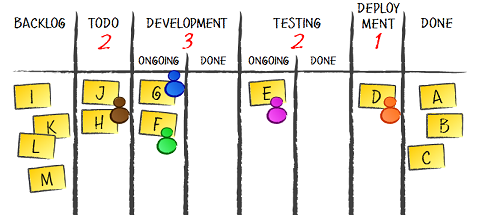
\includegraphics[width=1.0\textwidth]{img/kanban_board.png}
    \captionsource{Image showing the basics of a Kanban board. The cards move from left to right. The number under each category represent the \gls{wip} limit. }{Pawel Brodzinski, \url{http://brodzinski.com/}}
    \label{fig:kanban_board}
\end{figure}



\subsection{Visualize}
\label{sec:kanban_visualize}
This practice is about visualizing workflow. To have transparency between developers, managers and anyone else connected to a project. The standard way of doing this is using a so called Kanban board with cards, see Figure \ref{fig:kanban_board}. This board can either be a physical board with sticky notes, or a virtual board. This board is a visual control system for all the tasks within a project. The board allows for self-organizing by just pulling a new available card after finishing a task instead of waiting for a superior to supply the tasks.

The cards are not only meant to simply hold programming tasks. They are meant to represent some customer value. Therefor the design of the cards is important in order for the developers to make easier decisions on what to work on next. There are no exact rules on what information the cards should hold but a title, description, estimated size and some estimated value number is a good start \cite{key16}.

\subsection{Limit Work-in-Progress}
Limiting \gls{wip} is about having a limit at each step in the product chain, shown in Figure \ref{fig:kanban_board}, that corresponds to the amount of tasks allowed in that step. A simple \gls{wip} limit is having it equal to the amount of available working people at each step. When deciding the \gls{wip} limit, all members from from the \glspl{stake} to the developers should take part and form an agreement�\cite{key16}. 

The \gls{wip} limit is important for several reasons. It shows when a pull from one step can be made to the next. It ensures focus on one or a few tasks at a time. It keeps the workload balanced and avoids stock piling of items at some middle step in the product chain. The most important benefit is that it gives the development team a limit to rely on and fall back to when put under too much stress, especially if everyone participated and formed a consensus when choosing the limit for the \gls{wip}. 

\subsection{Manage Flow}
In Kanban the workflow or task flow is central so it makes sense having a practice focus on how to manage and improve it. In order to improve the workflow one must first be able to measure it somehow. Otherwise when changes are made, how do we know that it was an improvement? Some things are easier to measure and improve such as items stock piling at a certain step. An easy fix would be to add more manpower to that particular step. Some software such as \emph{Kanbanery} offer automatic tools for measuring that can give useful information about how changes affect the workflow \cite{key18}. Something important to stress out is that the more precise the estimated complexities and values for the cards/tasks the easier it gets to analyze the workflow.

\subsection{Make Process Policies Explicit}
In the practice Visualize the importance of having a clear design on the cards of the Kanban board was mentioned. This practice is about just that. Without clear rules and a common understanding of how the card system works the discussions becomes subjective and emotional instead of factual \cite{key19}. Having the Process Policies explicit makes them easier to understand and therefor easier to use. They help choices regarding the process become more rational and empirical and the team have an easier time reaching consensus simply because everyone is working from the same policy configuration.

The Process Policies are rules and procedures of the project, with focus on the Kanban board. It can state the type and amount of data that each card should contain. It explains the flow of cards traveling across the board. It can contain default implementation details about different classes of cards. The Process Policies basically defines the structure of the Kanban board and its cards.

\subsection{Improve Collaboratively}
\label{sec:improve_collaboratively}
\epigraph{If you are not continually improving, but you are doing all of the other parts of the Kanban method, you are missing the point. It's a little like the concept of "doing" agile but not being agile.}{\textsc{Matthew Powell} \cite{key19}}

\noindent
This practice is more social and less practically oriented than the others. When reading about Kanban you sometimes stumble upon the word \emph{Kaizen} meaning continuous improvement. \emph{Kaizen culture} is also often mentioned that talks about empowering the workforce and encourage them to "do the right thing". Kaizen culture promotes high levels of collaborations and freedom to self-organize work. It is about putting the company and business first and this requires lots of trust which Simon Sinek talk about in his TED Talk about leadership \cite{key7}.

Kanban promotes using a scientific approach when trying to introduce new changes. That means to evaluate a situation, suggest suitable change, predict the outcome, observe the results and compare with the prediction and previous results. If the team or business have a Kaizan culture together with using the scientific approach then that can lead to spontaneous and regular local improvements to the process \cite{key16}.

\section{Other Mentionable Methodologies}
\label{other_methodologies}
The informed reader might wonder why only these four methodologies were chosen for the report. After all there are at least a dozen more agile methodologies worth mentioning. For instance Dynamic Systems Development Method (DSDM) that is a broadly used agile methodology. 

The reason for the chosen methodologies are several. First of all we must acknowledge that going through every possible agile methodology is simply not possible. Kanban was chosen since it is both broadly used and very lightweight, making it a perfect choice for testing agile methodologies in small development teams. Crystal Clear was chosen as it clearly tries to address small development teams in its definition and there are not many agile methodologies that does so. Scrum is the most popular agile methodology today and therefor deserves a spot. \gls{xp} was chosen since it is popular but still quite different from the other methodologies, making it interesting for comparison reasons. 

DSDM was skipped simply because its scope is too large, larger than Scrum for example. This makes it impractical for this report since it talks about business cases and sponsorship which might not be the number one priority for small development groups. Feature-Driven Development (FDD) is another popular methodology but it has focus on big projects by discussing things like automated build systems. Some other methodologies are Adaptive Software Development (ASD), Scaled Agile Framework (SAFe), Disciplined Agile Delivery (DAD), Projects in Controlled Environments (PRINCE2) but they were all skipped for similar reasons, or lack of documentation. 



%\mypart{Method}{The method is divided in two chapters. The first chapter theoretically evaluates the agile methodologies in how well they would suite small projects and/or development groups. The project specification is also described here. At the end of the chapter a methodology is selected for the project. The second chapter is about the project workflow. It is a diary like evaluation of the selected agile methodology and the work progress.}

\chapter{Methodology Evaluation}
\label{sec:method_teori}
This chapter aims to theoretically compare the four agile methodologies to each other with focus on small development teams. At the end one methodology is selected to be used for the project, see \fullref{sec:project_description}.

There is no exact definition of what a "small project" or "small team" means. For the sake of clarification and consistency it is assumed that a small project consists of two to five member(s). They can either all be part of the development team or one or two have other responsibilities such as being a costumer, project leader or product owner. We further assume that the small team is within a small IT company and not some sort of small project team within a larger company. For example, it could be a handful of friends starting an IT consulting business after getting their master's degree in computer science. So whenever a small company, small project, small team etcetera is mentioned from here on, this is the setup to have in mind.

For the reader that skipped some parts of the prior chapter, it might be interesting to read \fullref{other_methodologies} that explains how the four methodologies were selected.

\section{The Agile Principles for Small Teams}
The agile principles are the backbone of agile development. Therefor it is only natural to compare agile methodologies to these principles in order to estimate how agile they are and what their differences are. However the principles aim to satisfy big projects and big teams since after all, the bigger the project the bigger the need for a methodology. Even if it is hard valuing the agile principles, or not even meant to by the founders and followers, it does make sense to reestimate their value for small newly started IT companies. The following evaluation of the principles is just an estimation based on logical reasoning and should be read with a critical mindset. The principles are listed at \fullref{sec:agile_principles}.

The first three principles regarding satisfying the customer, welcoming changing requirements and delivering software frequently feel equally important no matter the size of the project team. The fourth principle however, about business people and developers working together daily, is often naturally satisfied since in small projects they tend to be the same people. The fifth principle lowers greatly in importance since it is clearly focused on bigger companies where you can choose between different teams and people and give them projects to work with. As a newly started small company you kind of have to build the project around the hopefully motivated individuals. The only time face-to-face communication, principle 6, lowers in importance would be when you found a company or work on a project completely alone. Principle 7, 8, 9 and 10 all talk about keeping code quality high over time where the size of the project/company should not matter. Principle 11, which is about self-organizing teams, is pretty much self-fulfilling in a small new company. The last principle, number 12, is about team reflection and should be important in any sized project. 

To summarize, the 9 principles 1-3, 6-10 and 12 comes out as more important to satisfy than the rest for small new companies/teams. This short evaluation of the agile principles will help keep a better focus when evaluating the methodologies for small independent projects.

\section{Scrum}
The practices of Scrum satisfy the agile principles well. You can almost match each practice in Scrum to each different agile principle and perhaps this is why Scrum is often used as the example methodology for agile development.
The only principle that it does not address is principle 9 that talks about technical excellence and good design. Good code design is only briefly mentioned when talking about getting tasks done before the end of each Sprint and not leaving loose uncompleted ends. The methodology clearly revolves around the Sprints. It talks a lot about having short iterations with many short meetings and ensuring that the Product Backlog is kept updated at all times.

Everything in Scrum goes together pretty neatly as seen in Figure \ref{fig:scrum}. Each practice is strongly connected to several of the others. Within the events all three roles, the Scrum Master, Product Owner and Development Team described in \fullref{sec:roles}, work together tightly and always have the artifacts in focus. Generally this is a good thing since it shows coherence and makes it easier to grasp the meaning of each practice. However to be able to include all practices one would at least need three people to fill the roles. For the defined small project in this report, that would mean a Development Team of maximum three which can be a problem. An approach to get around this issue would be to have everyone part of the Development Team where two of the developers have extended roles as a Product Owner and Scrum Master. It is certainly possible to include all practices for a small project but it would also most certainly lead to lots of overhead work when so few people are involved.

\section{Extreme Programming (XP)}
\gls{xp} is quite opposite of Scrum and talks quite a lot about code quality. The practices Pair Programming, \gls{tdd}, Coding Standards, Simple Design and Refactoring all emphasizes how they have a positive influence on code quality. At first glance one might believe that \gls{xp} is much more "zoomed in" than Scrum and mostly talks about how the Development Team should code. However, the practice called The Planning Game is very big and includes components that are similar to several practices in Scrum, such as iterations (Sprints), small stories (Product Backlog) and planning meetings (Sprint Planning). So one could also see \gls{xp} as a sort of huge framework where Scrum is replaced by The Planning Game. So for companies using both Scrum and \gls{xp} it's a matter of perspective weather they are using \gls{xp} on top of Scrum or Scrum on top of \gls{xp}.

Since The Planning Game together with Small Releases is loosely put another version of Scrum, \gls{xp} satisfies the same practices that Scrum satisfies. The principle that Scrum did not satisfy, principle 9 regarding code quality, is quite clearly satisfied by many of the practices in \gls{xp}. Seeing how focused \gls{xp} is on code quality it is easier to understand the critique it receives regarding being called agile. After all, agile development is usually talked about in respect to cross-functional teams, short planning and regular meetings across the entire company hierarchy. 

\gls{xp} as a whole is quite clearly too extensive for small projects. They do however have many stand-alone practices that would be easy to start with and then slowly built upon, practice by practice. For example, all the quality ensuring practices mentioned. On the other hand, how agile would it be to have a bunch of practices satisfying only one agile principle? To ensure that the other parts of the agile principles are included one would have to look into the Planning Game. But instead of diving into that practice it would make more sense starting with Scrum where the different parts of The Planning Game are more clearly distinguishable.

\section{Crystal Clear}
Ironically the practices of Crystal Clear is the most vague of all four methodologies. They have chosen a higher abstraction on their practices, somewhere in between the agile principles and the practices of the other methodologies.  Instead of describing actual tools to achieve positive outcomes it focuses on describing positive outcomes with tools as examples. Half the practices, Osmotic Communication, Personal Safety and Focus, all talk about social behavior in group environments. The methodology revolves around building safety and trust within the team. In other terms, it has focus on the human mind instead of artifacts and processes. 

Since it has this high abstraction level it is hard to say which agile principles are touched. However the practices line of argument means that the more socially oriented principles 4, 5, 6 and 8 are being satisfied or are at least are in focus.

Crystal Clear is clearly more lightweight than \gls{xp} and Scrum which naturally means it would be an easier methodology to follow for small companies. To try to establish a sort of trust oriented culture early in a company, Crystal Clear is certainly a good candidate to follow. However it somewhat lacks practical practices to follow so it might be a good idea to complement it using another methodology or strategy. The methodologies Frequent Delivery and Reflective Improvement is basically the Sprint and Sprint Retrospective so Scrum would be a good candidate to pair it together with. 

The last principle, that certainly is more practical than the others, feels a bit malplaced. The way it is brought forward together with its content compared to the other practices, makes it sound more like general good coding tips than  
a practice within Crystal Clear.

One thing you can safely say is that Crystal Clear put heavy emphasize on the part of the The Agile Manifesto that states: \emph{Individuals and interactions} over processes and tools.
\section{Kanban}
Kanban is the most lightweight of the four methodologies. Like Scrum has a clear focus on the Sprints, Kanban has a clear focus on the Kanban board. It is only one of the five practices that does not revolve around the Kanban board, the practice Improve Collaboratively. It is so lightweight that it is arguable that Kanban is more of an agile/lean strategy than a complete methodology. As food for thought, the practices could be simplified and replaced 
by one practice called the Kanban Board. So it is not that strange that it is often mentioned when reading literature about Kanban that the methodology is meant to be expanded as time progresses and the project/company grows. 

Kanban certainly does not fully satisfy all the agile principles but the practices do nibble on almost all of them. For example principles 1-3 each have its own practice in Scrum that tries to satisfy them directly. In Kanban these are all incorporated though the Kanban board but in a more subtle way. Like with the other methodologies, except \gls{xp}, Kanban has no real focus on code quality. Also even if the Kanban board is about visualizing workflow for every member of a project it does not talk much about the collaboration between business people and developers. This means that principles 4 and 9 are left untouched. Other than that, Kanban seems to do have a covering but lightweight spread when it comes to satisfying the agile principles.

Kanban seems like a suitable choice to start with for a small new company looking for an agile methodology. It does a decent job covering the agile principles, it is relatively lightweight and most of the practices are easy to practically follow. However as a company/project grows it can perhaps become too lightweight and should be expanded or complemented using another methodology. An example of this is the methodology Scrum-ban which is a combination of Scrum and Kanban.

\section{Chosen Methodology}
Kanban became the chosen methodology for the project, see \fullref{sec:project_description}. There are several reasons for the methodology to be favorable for the project. The methodology covers most of the agile principles but is extremely lightweight compared to Scrum and especially \gls{xp}. For a small project this is essential since the smaller the project team the larger the overhead for a methodology. And in this particular project there will be just one developer and the owner of the project. Moreover, the fact that Kanban is meant to be expanded on demand and that methodologies like Scrum-ban exists, which is a combination of Scrum and Kanban, means that it should be easy to let the methodology grow as the project/company grows.

The Kanban board is easy to understand and implement. It will give value even if you are developing completely alone since it provides structure and abstraction. It also offers transparency for the project owner. The freedom of details on the Kanban board and its cards through the Process Policies means that it easy to start small and slowly buildup the organization of the board.

Regarding Crystal Clear, the focus on social environment makes it a pretty poor choice when working solo as a developer. Even if you are a handful of developers it can be hard to practically follow such abstract ideas. The methodology also does not have the same apparent coherency for its practices as the other methodologies which makes it feel fuzzy.

\chapter{The Project}
\label{sec:the_project}
This chapter has four sections. The first explains what the project is all about. The second section goes through the workflow of the project that has been developed using Kanban, and is at the time of this reports writing is still being developed. The third section goes through the practical results of the project. The final section is a short interview conducted with the product owner. 


\section{Project Description}
\label{sec:project_description}
This section is written in present tense to emphasize that it was the initial description for the project before any work had been conducted. Note that this was a real project and not just an experiment for this report. 

The project, to be developed using agile strategies, is a private initiative from Per-Arne Forsberg who has 25 years of successful international experience and knowledge in managing technically skilled units, products and projects around the world at Ericsson. Having been involved and engaged in change management, using the latest lean and agile methodology.

The project is developing a dynamic, scalable and robust interactive tutoring framework prototype for pre-academic students. Assisting students today according to the "old school" is social but also ineffective since it is usually one to one communication or one to a few in some geographical location (you have to meet at pre-determined location at pre-determined times, like classrooms). The long term goal is to assist in communication between students and teachers (tutors willing to help out with their knowledge from their preferred location) in Sweden and in turn combat the negative (knowledge) grade curve that can be seen around the country, according to international studies, PISA. 

In short the idea is to create an interactive website that can be used for many to many type of communication between students and teachers. An exact specification of the project does not exist in order to encourage the agile development process. 

\section{Working Agile}
This section goes though how agile development techniques were utilized for the project, especially how Kanban was used. It tries to follow a natural flow but does not follow a strict timeline. This is to improve readability and since the components of the development process were themselves developed over time, as for example the Process Policies, it makes sense to go through each component one by one.

\section{Timeboxing}
\label{sec:timeboxing}
Since the project was a private initiative by the product owner, the developer worked from his home. This was a problem since it impeded the collaboration between the two when they didn't get to see each other regularly face to face. To combat this timeboxing was used. Timeboxing is a term often used within agile development that means having fixed time periods where each period has its own budget, deadline and deliverables. Sprints in Scrum is for example a timeboxing technique, see \fullref{sec:scrum_events}.

Kanban does not talk about timeboxing. Mostly because when using Kanban to its full extent, it should not be needed. Complexity and scope variables, together with prioritization, for each work item in Kanban should be enough to estimate how many items will be completed within a certain timespan. In this project however, the developer was unexperienced working on web based projects, he worked alone and the time period for the project was only a few months. Therefor it made sense to use some sort of timeboxing instead of guessing complexity variables that would likely not be good estimates until the end of the project.  

The timeboxing used within the project was simple. Every tuesday at 10:00 the developer and product owner met for two to three hours and the items to be completed until next tuesday were selected. In other words, a fixed time period of one week was selected. Secondary items were also selected in case development went smoother than expected. If the goal wasn't reached this was discussed and information was added to the cards. Sometimes this led to cards being split into several items and sometimes the cards were simply moved to the next weeks deadline with the added information. Deadlines not reached were never seen as a failure, instead they were viewed as a learning experience to be able to better estimate workload in the future. This correlates well to the Kanban practice seen in \fullref{sec:improve_collaboratively}.

Besides estimating a weeks worth of work, the meetings were used to iteratively update the cards on the Kanban board which is brought up in \fullref{sec:kanban_cards}. During the course of the project extra meeting times were sometimes added, especially at the start of the project to get the ball rolling. 

\subsection{Process Policies}
One of the first things that was looked into, after deciding on using Kanban, was the layout of the Kanban cards, in other words the Process Polices. Typically these cards are either simply tasks and/or \glspl{us}. Since Kanban itself does not explicitly state the layout of the cards, the strategies described in Use-Case 2.0 were selected to form the basic structure \cite{key25}. This will be described further in \fullref{sec:use_case}.

Each card type got it own set of rules to follow, see figure \ref{fig:process_policy_sample}. Whenever a card was made it was checked against these rules to make sure it followed the defined structure. Moreover, the Kanban board had several rules and procedures connected to it such as that every item in the Done column waits for inspection at the next meeting. All of these rules and procedures were written in a card called "Rules / Process Policies" that can be seen in most upper left card in Figure \ref{fig:trello_kanban_board}. This ensured that they were always clearly visable.

All the projects Process Policies of the card are written in \appfullref{app:project_process_policies}, which is a mix of Process Policies connected to Use-Case 2.0, Kanban and more. The Process Policies were not all written at one point in time. As the project grew more policies were added. As soon as new procedures and rules were developed or discovered they were written down, some were however not written in text form for various reasons. For example the timeboxed meetings every tuesday. 

\begin{figure}[h!]
  \centering
    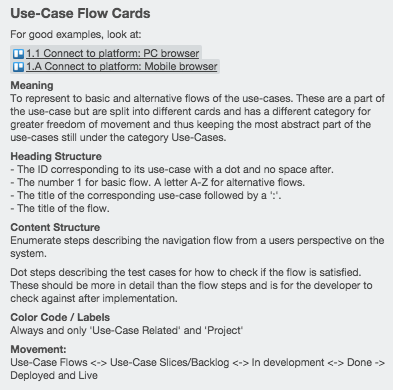
\includegraphics[width=0.67\textwidth]{img/process_policy_sample.png}
    \caption{A sample of the projects Process Policies. This sample shows information regarding the type of cards called Use-Case Flow Cards. For a full list of the Process Policies, see \appfullref{app:project_process_policies}.}
    \label{fig:process_policy_sample}
\end{figure}

\subsubsection{Use-Case 2.0}
\label{sec:use_case}
\Glspl{us} is a common approach in agile development to represent project requirements and specifications in a easy to understand, abstract and layered structure. A use-case is a similar alternative approach. The difference is in the scope and its focus. While \glspl{us} tend to be more abstract and use everyday language to keep it open for interpretation, use-cases instead are more user-to-system goal focused and tend to use a more business oriented language. Use-cases also tend to have larger scope that includes components such as \gls{uml}. It is common that project requirements are built using both \glspl{us} and use-cases techniques in some sort of combination. What's Important to know is that the definition for both of these techniques are not strict in order to have an easier time adapting them to any project type and size.

Use-Case 2.0 is a popular technique meant to be lightweight, scalable, versatile and easy to use \cite{key25}. If it delivers what it promises it sure fits the description of what to look for in a small project with few members. Also the technique is meant to be used with methodologies such as Kanban and Scrum. Without going into too much detail the technique, when used with Kanban, can be summarized as following:

\begin{enumerate}
\item Agree on the goals and scope of the system and identify all actors and ways of using the system. Repeat this regularly as things can change as the project develops.
\item Each use-case represents a meaningful logical interaction between some actor and the system.
\item Create a narrative for each use-case that explains the actors goal and interaction on an abstract level and in everyday language, similar to how \glspl{us} are written.
\item Create basic and alternative flows for each use-case that in a step-by-step manor goes through a users perspective in navigating the system to achieve the use-case goal.
\item Create basic test cases for how to check if the use-case and use-case flows are satisfied. 
\item When development on a use-case grows "near", as in actual implementation is soon to come, create slices for the use-case. As the name suggests, try to create each slice so they correspond to a suitable and somewhat equally sized work. The slices are created by either splitting a use-case flow or combining multiple flows. The slice can also go deeper in detail if wanted or needed, both in terms of the use-case flow steps and test cases.
\item Work on a certain number of slices at a time (depending on the size of the project team) and when implemented, check them against the test cases.
\item Keep updating the use-cases with information as slices are completed. 
\end{enumerate}

Note that this is a simplified summarization of Use-Case 2.0 that is influenced by both Kanban and the project. Read more about how to technique works in in the e-book \emph{Use-Case 2.0, The Guide to Succeeding with Use Cases} by Ivar Jacobson, Ian Spence and Kurt Bittner \cite{key25}.

\subsection{Kanban Board}
\label{sec:kanban_board}
\begin{figure}[h]
  \centering
    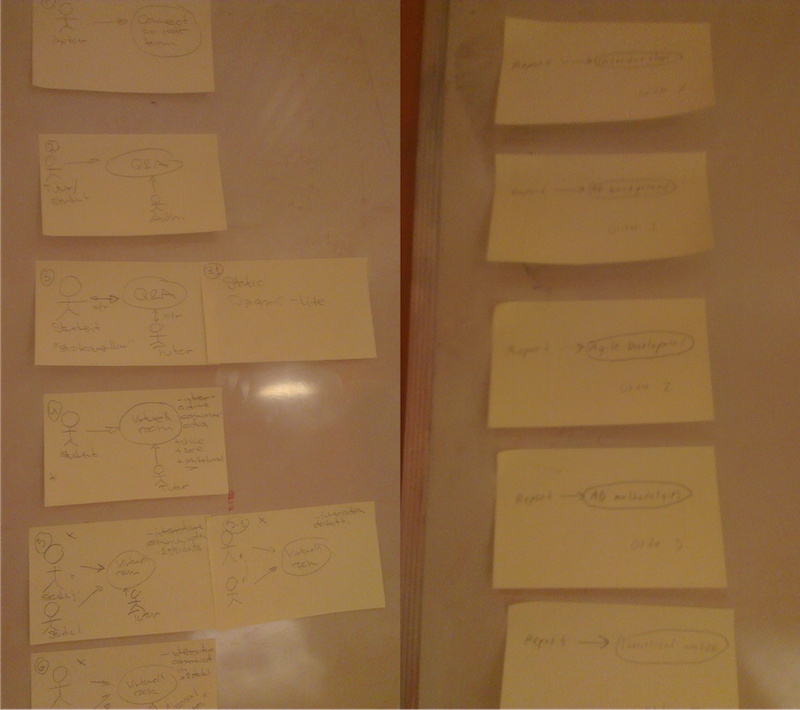
\includegraphics[width=0.9\textwidth]{img/post_its.png}
    \caption{Two combined pictures of the earliest stage of formulating use-cases. The left image shows the use-cases of the project where the most important components are already visible. The right side shows the initial use-cases for the report. The author sends his apologies for the poor image quality.}
    \label{fig:post_its}
\end{figure}
After deciding to use Kanban together with Use-Case 2.0, about five longer meetings corresponding to almost three full work days were spent on brainstorming the use-cases for the project. Each use-case was represented by a card and each card was a post-it note on a physical blackboard. These brainstorming sessions were kept highly abstract with focus on detecting the most important components of the project as well as all necessary components to make the website prototype a reality. This early stage of the project can be seen in Figure \ref{fig:post_its}. 

The physical blackboard became highly impractical as progress was made. The cards had to be taken up and taken down at every meeting since meetings took place at different public locations. Also overview became blurry with the use of only colored pencils and manual card linking. The most devastating issue was that modifying the content became a hassle and being able to easily change and modify the requirements is one of the most important aspects of agile development. So it was decided to move on to a virtual Kanban board. Many online options exists such as Kanban Tool, Kanbanize, Trello, Kanbanchi, SmartQ and many more. The selected online tool became Trello with the main reasons being that it is well established, free, lightweight and very easy to use. The advanced tools offered by the other options were not needed for a project of just two people. 

The Kanban board within Trello quickly became the center of the project and the center of attention at every meeting. All problems with the physical Kanban board were gone. Figure \ref{fig:trello_kanban_board} shows how the board looked after about three months into the project. As explained in the picture, only a few of the standards columns in Kanban were used. The reason being to limit overhead when only one developer is working on the board. For example, the backlog and todo columns are combined and also testing is assumed to be done before moving to column Done and once again tested at a meeting before moving to Deployed and Live.  

\begin{figure}[h]
  \centering
    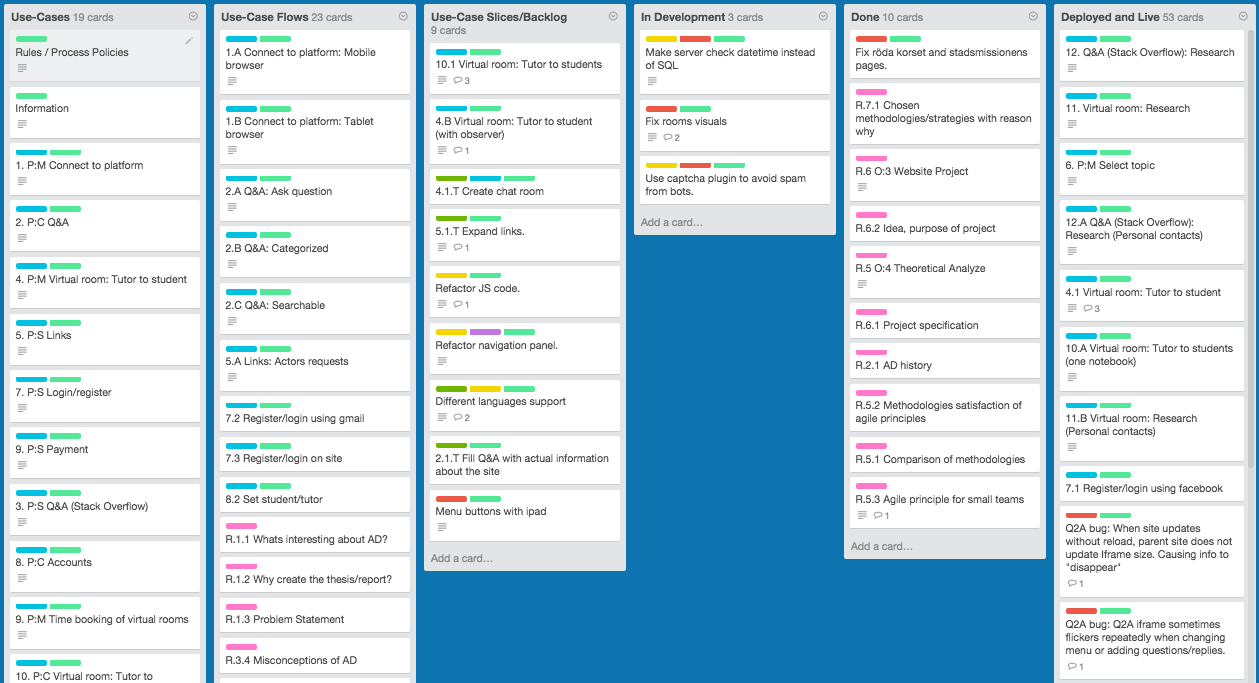
\includegraphics[width=1.0\textwidth]{img/trello_kanban_board.png}
    \caption{A part of the Kanban board used with the online software tool Trello: \url{https://trello.com/}. The three most left columns are part of the Use-Case 2.0 strategies. The four right columns are the most basic steps used within Kanban that somewhat corresponds to the columns seen in Figure \ref{fig:kanban_board}. The third column is both a part of the Use-Case 2.0 strategies and a standard Kanban step.}
    \label{fig:trello_kanban_board}
\end{figure}

\newpage
\subsubsection{Kanban Cards}
\label{sec:kanban_cards}

\begin{wrapfigure}{r}{0.45\textwidth}
	\captionsetup{font=scriptsize,labelfont=scriptsize, singlelinecheck=false, labelfont=bf}
	
	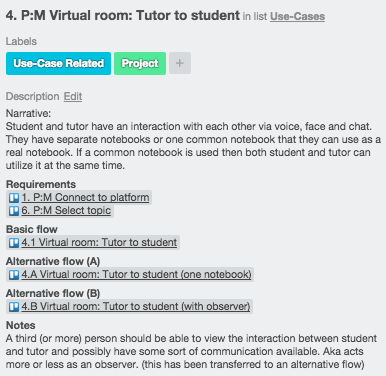
\includegraphics[width=0.45\textwidth]{img/use_case_card.png}
	\vspace{-14pt}
  	\caption{Example of a Use-Case Flow Card.}
   	\label{fig:use_case_card}
   	\vspace{12pt}
   
   	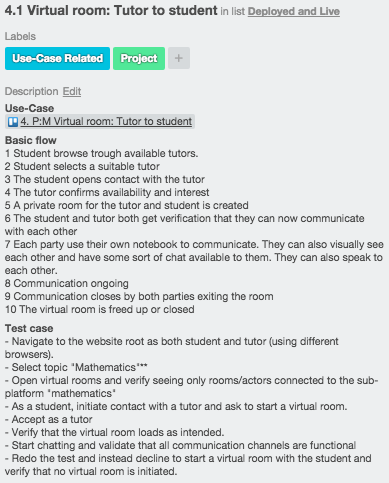
\includegraphics[width=0.45\textwidth]{img/use_case_flow_card.png}  
	\vspace{-14pt}
   	\caption{Example of a Use-Case Flow Card.}
  	\label{fig:use_case_flow_card}
   	\vspace{12pt}

   	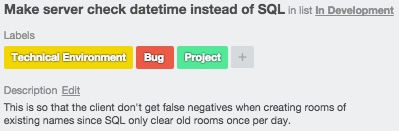
\includegraphics[width=0.45\textwidth]{img/task_card.png}
   	\vspace{-17pt}
  	\caption{Example of a Task Card.}
  	\label{fig:task_card}
\end{wrapfigure}

An example of the structure policies, or rules, for the cards can be seen in Figure \ref{fig:process_policy_sample}. The card types are Use-Case Cards, Use-Case Flow Cards, Use-Case Slices Cards, Task Cards and Report Cards. To understand how these exactly work it's best to look at \appfullref{app:project_process_policies}.

Close to everything about the project was written inside the cards. Every task or idea had a card connected to it. The cards has basically three movement types after creation: It can move its way to the right on the board until it ends up in Deployed and Live. It can at some point in some category be removed, or archived as it is called in Trello, if it is found unwanted. These cards are not permanently deleted and can always be found again after removal. Finally a card can find itself to be frozen in some category, except in In Development and in Done. The cards in Deployed and Live are for instance normally frozen in place. Other examples are low priority cards in the Backlog or earlier categories that have a small value but high complexity.  

At each meeting, new cards could be created or existing cards could be modified. It was during the meetings that it was decided which cards should be kept, removed or worked on for the coming week. Also the cards in the Done column were tested and discussed together with the cards in the In Development column. Another important part of the meetings were organizing the Backlog column so that the cards were kept arranged in priority order from top to bottom.

The Report cards are special. They were added early since the author of report and the developer is the same person. Therefor it made sense including these cards since it gave the product owner a better overview of what was going on at every meeting. After all, one of the practices in Kanban is about having transparency in a project, see \fullref{sec:kanban_visualize}.

\section{Project Results}
\label{sec:project_result}
\begin{figure}[h]
  \centering
    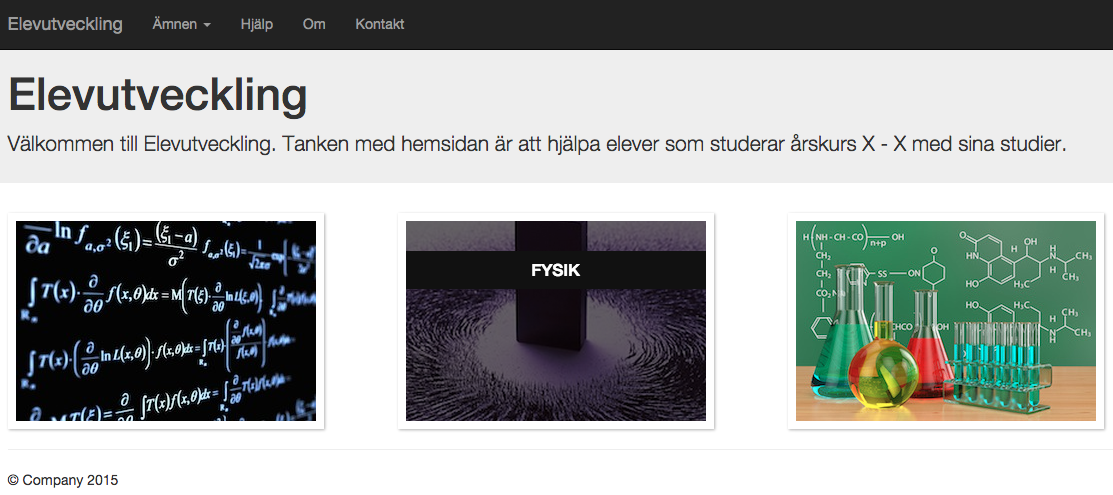
\includegraphics[width=1.0\textwidth]{img/elevutveckling.png}
    \caption{The home page of the website prototype showing three selectable images for school subjects. Mathematics, physics and chemistry. The mouse is hovering over physics. At the time of this reports writing the website can be found at: \url{http://elevutveckling.com/} }
    \label{fig:elevutveckling}
\end{figure}

Drawing any conclusions regarding how much Kanban assisted the project in terms of quality is complicated, which is discussed in \fullref{sec:discussion}. However a part goal of this thesis was to develop a working prototype of the interactive website and this chapter shows where the project landed in that regard.

The goals for the prototype were initially set after the projects use-cases were identified, as described in \fullref{sec:kanban_board}. However since the use-cases contents changed, as the project developed, the definition of the goals also changed. As The Agile Manifesto states, \emph{Responding to Change over Following a Plan}. Excluding the most basic features, such as having a functional navigation, the final required functionality for the website to be counted as a working prototype became these three use-cases:

\begin{description}
\item[1. Virtual room: Tutor to student] \hfill \\
The most important use-case. For each subject, a student and a teacher must be able to enter a virtual room together containing a virtual whiteboard. The whiteboard should function as a regular whiteboard where the student and teacher can draw equations and do calculations. All three communication channels, video, voice and chat, must be available. 
\item[2. Q\&A (Stack Overflow)] \hfill \\
Each subject must have question and answers section, similar in functionality as the well known website called Stack Overflow. The students must be able to ask questions, find questions and answer other students questions related to the subject they are currently navigating in. 
\item[3. Links] \hfill \\
The least complicated of the three required use-cases. Each subject must have a range of interesting external links connected to the studying of that subject.
\end{description}

Note that these descriptions are the most basic requirements for the prototype and the actual use-cases contains more information as seen in Figure \ref{fig:use_case_card} and \ref{fig:use_case_flow_card}.

\subsection{Project Components}
This section will show the more abstract components used in the project to create the website as for example what frameworks were used.

\begin{description}
\item[Git] \hfill \\
Of course the some sort of code management and version handling system were to be used in the project, as every project should have. Git was chosen as it is a popular and well established code management system that the developer had prior experience working with. The online Git framework Github was used to offer a better visual experience. \url{https://github.com/}
\item[Misshosting] \hfill�\\ 
The web hotel used for the website. Used simply for having the servers in Sweden together with the fact that it uses cPanel which is a popular user friendly graphical web hosting control panel, which makes the website easier to administrate for people inexperienced in web development. MySQL was used for the database. \url{https://misshosting.se/}
\item[Bootstrap] \hfill \\ 
Bootstrap is a well established comprehensive design framework using \gls{css} and Javascript. It was used to let the developer, who has little experience in design, focus more on functionality. Besides giving a sleek design it is responsive in such a way that the website looks and functions well on different resolutions such as those found in phones. Because of its popularity it also has many useful plugins such as the form validation plugin called Bootstrap Validator that was used in the project. Thus utilizing Bootstrap, or similar frameworks, means avoiding reinventing the wheel. \url{http://getbootstrap.com/}
\item[Groupworld] \hfill \\ 
One of the earliest use-cases looked into for the project was conducting a research in order to find suitable frameworks, or platforms, to satisfy the virtual room use-case, as described in \fullref{sec:project_result}. Besides the developer doing a research, a third party company was used to help in the investigation which led to the finding of Groupworld, see \appfullref{app:virtual_room_research}.

Groupworld is a highly customizable cross-platform web conference platform for online meetings using video, voice and chat. The most important feature of the platform is that it integrates smoothly to existing websites. The result of the integration can be seen in Figure \ref{fig:groupworld}. \url{http://www.groupworld.net/}

\label{sec:project_result}
\begin{figure}[h]
  \centering
    
\includegraphics[width=0.8\textwidth]{img/groupworld.png}
    \caption{Image showing the groupworld platform integrated with the website. The whiteboard in the middle can be used with features shown to the right, similar to Microsoft Paint. The plugins above offers mathematical support such as writing the sample integral equations visible in the whiteboard. The connected users can see each other, talk to each other and also chat using the chat window at the bottom. All three users is the developer himself, which is the reason for the duplicate video channels to the left.}
    \label{fig:groupworld}
\end{figure}

\item[Question2Answer] \hfill \\ 
A framework used to satisfy the second most important use-case requirement for the website prototype, explained briefly at \fullref{sec:project_result}. A initial research was conducted to find suitable frameworks, like with the virtual rooms, but without using a third party company. Question2Answer was the picked solution. Besides satisfying the basic requirements, it also offers support for voting, structuring, ranking system and more. It is popular and open source which both were favorable qualities for the project. Since the framework is meant to function as a stand alone website it was stripped down to the most essential components and integrated with both Bootstrap and the project website. The result of the integration can be seen in Figure \ref{fig:subject_page}. \url{http://www.question2answer.org/}

\label{sec:project_result}
\begin{figure}[h]
  \centering
    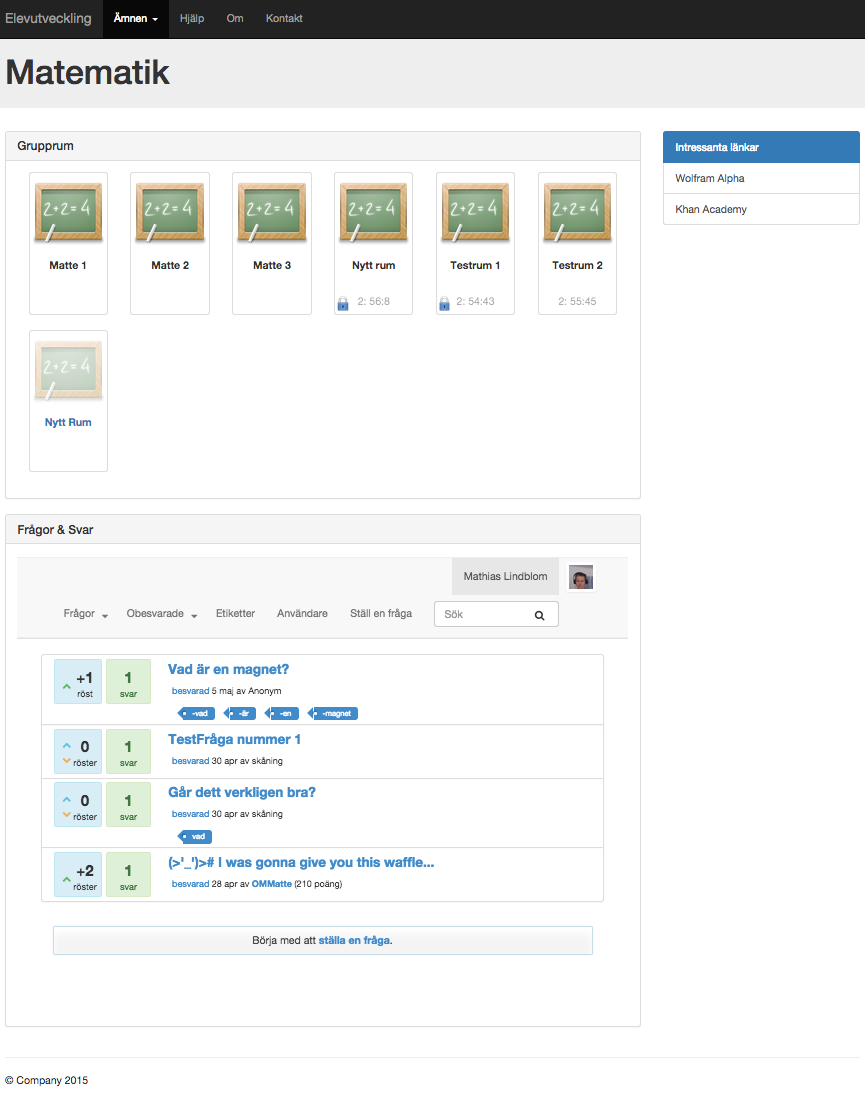
\includegraphics[width=0.71\textwidth]{img/subject_page.png}
    \caption{Image showing the page of a subject, mathematics to be precise, in the website prototype. Below the page title the virtual group rooms can be seen. Some are password protected while others are publicly open. Some also have a timer which shows how long the rooms stay up before they disappear. Anyone can create a new room using the "Nytt Rum" (English: New Room) icon. At the bottom the Question2Answer framework can be seen integrated with the Bootstrap layout. To the right are links to external helpful sites regarding studying mathematics. In other words, the image shows all three required components described in \fullref{sec:project_result}.}
    \label{fig:subject_page}
\end{figure}	

\item[iHover] \hfill \\
A image framework used for styling and effects. Used for the websites navigation images, seen in Figure \ref{fig:elevutveckling}. Integrates well with Bootstrap. \url{http://gudh.github.io/ihover/dist/}

\end{description}

\section{Product Owner Experience}
\paragraph{What worked well using Kanban?} \hfill \\ 
Getting a solid structure. I could clearly follow how the project developed over time. It was easy keeping track of the status of the development process.

\paragraph{What did not work well using Kanban?} \hfill \\ 
I thought it worked really well actually, can not think of anything directly bad or not working. Maybe that without the timeboxed meetings, that were not a part of Kanban, Kanban might have felt a bit thin.

\paragraph{Did Use-Case 2.0 bring any value to using Kanban?} \hfill \\ 
Yes, it worked well to use it together with Kanban, especially since it was hard for us to know how long time the different components would take to develop. Use-Case 2.0 made it easy to break down the components to more manageable pieces. After the break down it was easier to analyze and adapt the components to the Kanban board.
\paragraph{Do you think Kanban was advantageous to the project?} \hfill \\ 
Yes. I don't know any other agile methodology that could replace Kanban for this kind of work. Not any other type of methodology either for that matter. Nothing I know of would offer the same kind of transparency to a project, all the way from the early stages to delivery. Moreover, the methodology offered great flexibility which was important in this project.
\paragraph{What are your thoughts on the collaboration between you and the developer in regards to using Kanban? Both positive and negative thoughts.} \hfill \\ 
As I said, the transparency and structure was great and I could easily follow the work flow. We were open and clear to each other and the board helped in that regard. I could easily follow the developers progress. This made it easy to reprioritize and restructure regularly. Even the individual components progress were easy to track where they were in their development phase. Don't really have any negative thoughts.

\paragraph{What would you like to have done differently, given the opportunity to redo the project?} \hfill \\ 
Nothing, or wait. Remove all report writing. Every sentence in the report was one functionality lost in the project. 


\paragraph{What is your final verdict to using Kanban in the way it was used in the project?} \hfill \\ 
It worked very well. As stated in the other questions, it gives transparency, structure and flexibility.

\paragraph{Would you recommend this projects methodology approach for similar projects?} \hfill \\ 
I recommend to use this methodology when designing new projects with a small group of participating people. Especially when the initial requirements leaves many unknown parameters.
\paragraph{Any final thoughts?} \hfill \\ 
No, just that I think the project went very well overall.



%\mypart{Discussion}{The following chapters will be discussions and final toughs regarding the results, future work, report critique and more.}

\chapter{Discussion}
\label{sec:discussion}
The first thing to mention is that it was initially planned to be three developers on the project. Three developers, or at least two, would mean that more agile practices could have been tried out since most of the practices are about communication between the project members. It would also mean that the report writer could have had a greater focus on agile development and spend less time coding.



\section{Conclusions}

\section{Report Critique}
There are several reasons to be critical for the type of research conducted in this report. Some have already been mentioned briefly here and there throughout the report. The first thing to note is that agile development by itself is quite vague in its definitions and the work regarding agile development and its methodologies are mostly based on expert experience. It is the results of industry experts that have seen problems, come up with ideas to fix them, had companies or themselves try them out and finally evaluate the outcome. The problem is that there are so many parameters and influences when evaluating software development methodologies that it is really hard to make sense of the result. Too be clear, the data is very noisy. For instance, you can not make a software using one methodology and then have the development team create the software again using another approach. The results of the new approach will most certainly be influenced by their first attempt. What is really needed is several development teams consisting of developers with somewhat equal experience and background. However, depending on parameters such as if the software type is a website, game or security system the results might vary. Thus most work regarding agile development and its methodologies, including this report, falls into the category of social science or soft science which is important to have in mind. All of this also means that investigating work regarding agile development, such as this report, would benefit in having a more experienced author but this is usually hard to come around when we talk about a university thesis for obvious reasons.

Each agile development methodology has vast amount of information, interpretations and alternative versions going for them. To make a full theoretical analyzes and comparison is out of scope for this report. The first and easy limitation was to not include every possible agile methodology in order to have room for more depth into the chosen methodologies as well as to keep the complexity down. The reasoning behind the four chosen methodologies can be read at \fullref{other_methodologies}. However, even with this limitation it would not be viable going through every aspect of each methodology since each methodology deserves their own full report. So the practices of each methodology was chosen as a solid and common ground to be analyzed. What this means is that a lot of what defines the methodologies have potentially been "cut off" and therefore given an unfair assessment to some degree. This is also brought up in \fullref{sec:future_work}.

\section{Future Work} 
\label{sec:future_work}


\printglossary[type=main]
\nopagebreak[4]
\printglossary[type=\acronymtype]


%\appendix
%\addappheadtotoc
%\chapter{RDF}\label{appA}

\begin{thebibliography}{56}

\bibitem{key1}
Martin, C.R. and Martin, M. 
2006. 
Agile principles, patterns, and practices in C\#. 
Prentice Hall, Massachusetts. 
768 pp.

\bibitem{key2}
Agile Alliance. 
2015. 
The alliance. 
[ \url{http://www.agilealliance.org/the-alliance/} ]. 
Accessed Mars 5, 2015.

\bibitem{key3}
Crockford, C. 
2007. 
Quality. 
[ \url{https://www.youtube.com/watch?v=t9YLtDJZtPY&t=175} ]. 
Accessed Mars 12, 2015.

\bibitem{key4}
Knuth, D.E. 
1984. 
Literate Programming. 
Comput J. 
27: 97-111. 
%\url{http://www.literateprogramming.com/knuthweb.pdf}

\bibitem{key5}
Cockburn, A. 
2004. 
Crystal clear: a human-powered methodology for small teams. 
Addison-Wesley Professional, New Jersey. 
312 pp.
% \url{http://users.dcc.uchile.cl/~nbaloian/cc1001-03/ejercicios/crystalclearV5d.pdf}

\bibitem{key7}
Sinek, S. 
2014. 
Why good leaders make you feel safe. 
[ \url{http://www.ted.com/talks/simon_sinek_why_good_leaders_make_you_feel_safe} ]. 
Accessed Mars 13, 2015. 

\bibitem{key8}
Keil, M. and Carmel, E. 
1995. 
Customer developer links in software development. 
Commun ACM. 
38: 33-44.

%\bibitem{key9}
%[Cockburn2001] Alistair Cockburn and Laurie Williams, "The Costs and Benefits of Pair
%Programming," XP2000 Conference in Sardinia, reproduced in Giancarlo Succi and Michele Marchesi,
%Extreme Programming Examined, Addison-Wesley, 2001.

%\bibitem{key10}
%[Nosek98] J. T. Nosek, "The Case for Collaborative Programming," Communications of the ACM,
%1998, pp. 105108.

\bibitem{key11}
Williams, L., Kessler, R.R., Cunningham, W. and Jeffries R. 
2000. 
Strengthening the case for pair programming. 
IEEE Softw. 
17: 19-25.

%\bibitem{key12}
%\url{https://people.kth.se/~tomase/#/presentations/computer_science}

%\bibitem{key13}
%\url{http://repo.hackerzvoice.net/depot_madchat/coding/xp/xpexplained.pdf}

\bibitem{key14}
Beck, K. and Andres, C. 
2004. 
Extreme programming explained: embrace change, 2nd edition. 
Addison-Wesley Professional, New Jersey. 
224 pp. 
%\url{http://ptgmedia.pearsoncmg.com/images/9780321278654/samplepages/9780321278654.pdf}

\bibitem{key15}
Scrum Guides. 
2013. 
The scrum guide. 
[ \url{http://www.scrumguides.org/scrum-guide.html} ]. 
Accessed Mars 23, 2015. 

\bibitem{key16}
Anderson, D.J. 
2010. 
Kanban: successful evolutionary change for technology organizations. 
Blue Hole Press. 
278 pp. 
%\url{http://www.scrumsense.com/wp-content/uploads/2010/02/KanbanManuscript-dja-rev1_07_2.pdf}

%\bibitem{key17}
%\url{http://en.wikipedia.org/wiki/Kanban}

\bibitem{key18}
Klipp, P. 
2014. 
Getting started with kanban. 
Kanbanery. 
37 pp.
%[ \url{https://kanbanery.com/ebook/GettingStartedWithKanban.pdf} ]. 

\bibitem{key19}
Everyday Kanban. 
2015. 
What is kanban. 
[ \url{http://www.everydaykanban.com/what-is-kanban/} ]. 
Accessed Mars 25, 2015.

% \bibitem{key20}
%\url{https://www.google.se/books?%hl=sv&lr=&id=6O5tAgAAQBAJ&oi=fnd&pg=PR3&dq=scrum&ots=1FXoZqQl5Z&sig=oAaGuCqYT8GOPb3L4u6kqIoWYH8&%redir_esc=y#v=onepage&q=jeff%20sutherland&f=false} %About combining xp with scrum

\bibitem{key21}
Schwaber, K. 
2004. 
Agile project management with scrum. 
Microsoft Press. 
192 pp.
%\url{https://www.google.se/url?sa=t&rct=j&q=&esrc=s&source=web&cd=1&ved=0CCUQFjAA&url=http%3A%2F%2Fxa.yimg.com%2Fkq%2Fgroups%2F19611210%2F134287803%2Fname%2FAgile&ei=MXsRVeqRMeHXyQOJtoCoDA&usg=AFQjCNEBuHLF_m23E8qOTsBJvOtetCxukw&sig2=J3vpAfBnP0Mhms92bnycIA&bvm=bv.89184060,d.bGQ&cad=rja}

\bibitem{key22}
Womack, J.P., Jones, D.T. and Roos, D. 
2007. 
The machine that changed the world: the story of lean production. 
Free Press, New York. 
352 pp. 

\bibitem{key23}
Poppendieck, M. and Poppendieck, T. 
2003. 
Lean software development: an agile toolkit. 
Addison-Wesley Professional, New Jersey. 
240 pp.
%http://ptgmedia.pearsoncmg.com/images/9780321150783/samplepages/0321150783.pdf

\bibitem{key24}
Fowler, M. 
2008. 
Agile versus lean. 
[ \url{http://martinfowler.com/bliki/AgileVersusLean.html} ]. 
Accessed April 1, 2015.

\bibitem{key25}
Jacobson, I., Spence, I. and Bittner K. 
2011. 
Use-case 2.0.
Ivar Jacobson International.
55 pp.

%\bibitem{key25}
%\url{http://www.quotium.com/performance/comparison-of-key-methodologies-in-agile/}

\end{thebibliography}

\appendixname{Appendix}
% \cleardoublepage
%\addcontentsline{toc}{chapter}{Appendices}
\addtocontents{toc}{\protect\setcounter{tocdepth}{0}}
\begin{appendices}

\chapter{Project Process Policies}
\label{app:project_process_policies}
The Process Policies for the project are written in the online organization tool called Trello. For the time being they can be accessed using the following link: \url{https://trello.com/c/Xtm9s8LF/95-rules}

However since the project is ongoing the information will change and the link might become invalid in the future. A sample of how to Process Policies are written in Trello can be seen in Figure \ref{fig:process_policy_sample}. The Kanban board in Trello is visible at Figure \ref{fig:trello_kanban_board}. Everything below is an extraction of the Process Policies at the time of this reports writing, slightly modified to suit the layout of this report.


\section{Project Process Policies}
Strategies in Use-Case 2.0 are integrated with the Kanban board.

\subsection{General Kanban Board Policies}
\begin{itemize}
\item Normally the cards move from left to right on the board. Each card type has more information on this below.
\item The categories Use-Cases and Use-Case Flows are only for the Use-Case Cards and Use-Case Flow Cards. However, new ideas should be new cards in Use-Cases and discussed in the next meeting.
\item The Use-Case Slices/Backlog is the "To-Do" list that a developer can grab and move to In Development. The cards highest up are the most prioritized card.
\item Everything in In Development should be something being worked on by a developer. If the developer pauses work it should move back to the Backlog and if the work is done it should move to Done before grabbing a new card.
\item Before moving to Done, the developer should have run the tests described in a card. Even if no tests are written, testing should still be conducted.
\item Cards in Done await inspection before being moved back to the Backlog or being decided to put the code live.
\item At the next meeting. Each card in Done should be explained and tested once again before deciding if the card should be Deployed or not. The card must of course be put live by a developer before being moved to Deployed.
\item Cards only move to Deployed and Live from Done. The cards must also of course be deployed and live.
\end{itemize}


\subsection{Use-Cases Cards}
For a good example, look at: 

\url{https://trello.com/c/JvD4oEyF/47-1-1-connect-to-platform-pc-browser} 

\begin{description}
\item[Meaning] \hfill \\ 
To represent to most abstract part of the use-cases whose content could change greatly over time.

\item[Heading Structure] \hfill
\begin{enumerate}
\item Use-case ID, a unique number followed by a dot.
\item Priority following MoSCoW written "P:X" where 'X' is either M (Must), S, (Should), C (Could), W (Would).
\item Title name of the use-case.
\end{enumerate}

\item[Content Structure] \hfill \\ 
Begin with the narrative and use everyday language. What does the actor want to achieve? What is the goal of the use-case? Make sure it is clear who the actor is.

If requirements exist, leave a heading and link to each Use-Case Card or any other card that is a requirement. No need to implement already implemented cards.

Leave a heading for the basic flow and all alternative flows, if they exist. Link each flow to the card corresponding to that particular flow. 

Add any possible notes that are not related to the narrative in the end. Comments can also be used for notes. 

\item[Color Code / Labels] \hfill \\ 
Always and only 'Use-Case Related' and 'Project'

\item[Movement] \hfill \\ 
Use-Cases <-> Done -> Deployed and Live

The card sit still in Use-Cases and only move to done when all use-case flows corresponding to the card are moved to Done or Deployed and Live. Once there the decision is made weather or not it is truly satisfied and can either move back or to Deployed and Live. The card can also be Archived if decided to be unwanted.
\end{description}


\subsection{Use-Case Flow Cards}
For good examples, look at: 

\url{https://trello.com/c/JvD4oEyF/47-1-1-connect-to-platform-pc-browser}

\url{https://trello.com/c/4krVGIwA/48-1-a-connect-to-platform-mobile-browser} 

\begin{description}
\item[Meaning] \hfill \\ 
To represent to basic and alternative flows of the use-cases. These are a part of the use-case but are split into different cards and has a different category for greater freedom of movement and thus keeping the most abstract part of the use-cases still under the category Use-Cases. 

\item[Heading Structure] \hfill
\begin{enumerate}
\item The ID corresponding to its use-case with a dot and no space after.
\item The number 1 for basic flow. A letter A-Z for alternative flows.
\item The title of the corresponding use-case followed by a ':'.
\item The title of the flow.
\end{enumerate}

\item[Content Structure] \hfill \\ 
Enumerate steps describing the navigation flow from a users perspective on the system.

Dot steps describing the test cases for how to check if the flow is satisfied. These should be more in detail than the flow steps and is for the developer to check against after implementation. 

\item[Color Code / Labels] \hfill \\ 
Always and only 'Use-Case Related' and 'Project'

\item[Movement] \hfill \\ 
Use-Case Flows <-> Use-Case Slices/Backlog <-> In development <-> Done -> Deployed and Live

\end{description}

\subsection{Use-Case Slices Cards}
For a good example, look at:

\url{https://trello.com/c/Dpd63Jy0/114-5-1-t-expand-links}

\begin{description}
\item[Meaning] \hfill \\ 
These cards are Use-Case Slices or Use-Case Tasks that represents a part of a Use-Case Flow. It can either be a few exact steps of the flow, a task needed to satisfy the flow or a small addition to a flow deserving of its own card.

\item[Heading Structure] \hfill
\begin{enumerate}
\item The entire Use-Case Flow ID followed by no space.
\item The letter 'T'.
\item Title of the slice, or task.
\end{enumerate}

\item[Content Structure] \hfill \\ 
As you wish. The purpose of the card should be clear. However if the card is a strict part of some steps of a flow. Those steps should be written down.

\item[Color Code / Labels] \hfill \\ 
Always 'Project'.
Always 'Use-Case Related' if it is a strict subset of a Use-Case Flow.
Never 'Report'.
The rest are optional.

\item[Movement] \hfill \\ 
Use-Case Slices/Backlog <-> In Development <-> Done <-> Deployed and Live

These cards can be directly put to 'In Development'.

\end{description}

\subsection{Task Cards}
A good example:

\url{https://trello.com/c/5Mrp0crr/121-refactor-navigation-panel}

\begin{description}
\item[Meaning] \hfill \\ 
A task card does not directly correlate to a use-case and its flow(s). It can be a small feature, bug, design improvement etcetera. Basically anything that can add some form of value but does not fit logically to a use-case. If the complexity of card is large it should perhaps be converted to a Use-Case card.

\item[Heading Structure] \hfill \\
Just a fitting title of the task.

\item[Content Structure] \hfill \\ 
As you wish. Be as detailed as possible and needed.

\item[Color Code / Labels] \hfill \\ 
Always 'Project'.
Never 'Report' or 'Use-Case Related'.
The rest are optional.

\item[Movement] \hfill \\ 
Use-Case Slices/Backlog <-> In Development <-> Done <-> Deployed and Live.

These cards can be directly put to 'In Development'.

\end{description}

\subsection{Report Cards}

\begin{description}
\item[Meaning] \hfill \\ 
These cards are for the report writer and only he/she knows its meaning.

\item[Heading Structure] \hfill \\
As the report writer pleases.

\item[Content Structure] \hfill \\ 
As the report writer pleases.

\item[Color Code / Labels] \hfill \\ 
Always and only 'Report'.

\item[Movement] \hfill \\ 
As the report writer pleases.

\end{description}

\chapter{Virtual Room Research Results}
\label{app:virtual_room_research}
The following is the results from using a third party company to conduct research regarding finding suitable virtual room frameworks, or platforms, for the project. A platform called Groupworld offered by Group Technologies Inc became the selected platform for the website prototype, see number 7 in the included pdf on the next page.

\includepdf[pages=-]{pdf/virtual_room_research_results.pdf}

\end{appendices}

\end{document}


%Other mentionable Methodologies. H�nvisa till detta efter bakgrunden.

%Focuses heavily* skriv om have a strong focus

%Type of investigation, this type of. Skriv om

%next small abstraction step, tydligg�r, clarification

%This section will a short illut...

%called waterfall model

%the waterfall model takes on logical project step -> project will go through different phases sequential.

%L1, A1. F�rklara vid f�rsta anv�ndated.

%Newly founded => small companies

%The fourth  principle, tydlig�r att det inte �r mindre viktigt, utan att det kommer naturellt.

%This quick purge, lite mildare ordval.

%All three roles, 4.2. Skriv ut dom och h�nvisa.

%Scrum 4.2 skriv om sista delen.

%Vast -> extensive

%4.4 Sociallly focused agile principles

%nibble -> kanske �ndra

%Time boxed, f�rklara i  Using Kanban eller passande plats. Skriv i 4.6 p� slutet att andra tekniker utnyttjats tillsmannas med Kanban i chapter blabla.

%5.0 ...was and, at... skriv om.

%5.2 It tries to keep a natural flow but does not follow a strict timeline.

%Most of the policies -> All of the poicies. L�gg till punkt efter Process Polices. 


%Use Case 2.0 "now and then" -> on a regular basis.

grows "near", fundera ut ett alternativ

Kl�m in demos, att vi testar produkten regelbundet. Kanske i en ny rubrik (regular meetings)

% During development new cards were continuously created -> were created.

% Report writer -> author of the report. at every meeting -> within the project.

% 5.3 The goals for the prototype... L�gg till mening som f�rklarar att arbetsprocessen f�r�ndrade m�len.

%required componets -> required functioanlity

%CSS -> f�rkortning

%6.2 First of all

%readers some focus 6.2 ta bort

Time boxed meetings is not a standard practice in Kanban since it is assumed that you have a common workplace. In our project this was not the case so in order to ensure a tigher collaboration blablabal

Skriv vilka praktiker som satisfieras i Kanban
